%Este trabalho está licenciado sob a Licença Atribuição-CompartilhaIgual 4.0 Internacional Creative Commons. Para visualizar uma cópia desta licença, visite http://creativecommons.org/licenses/by-sa/4.0/deed.pt_BR ou mande uma carta para Creative Commons, PO Box 1866, Mountain View, CA 94042, USA.

\documentclass[12pt]{book}

%%% preambulo
\input ../preambulo.tex
\input ../preambulo_counters.tex
\input ../preambulo_python.tex

\ifispython
\lstset { %
  language=Python,
}
\fi

\makeindex

\begin{document}

\frontmatter

\title{Redes Neurais Artificiais}
\author{Pedro H A Konzen}
\date{\today}
\ifishtml
\else
\addcontentsline{toc}{chapter}{Capa}
\fi

\maketitle

% \nocite{Goodfellow2016a}

% licença


\chapter*{Licença}\label{licenca}
\addcontentsline{toc}{chapter}{Licença}

Este texto é disponibilizado sob a Licença Atribuição-CompartilhaIgual 4.0 Internacional Creative Commons. Para visualizar uma cópia desta licença, visite 
\begin{center}
  \url{http://creativecommons.org/licenses/by-sa/4.0/deed.pt\_BR} 
\end{center}
ou mande uma carta para Creative Commons, PO Box 1866, Mountain View, CA 94042, USA.




\chapter*{Prefácio}\label{prefacio}
\addcontentsline{toc}{chapter}{Prefácio}

O site \href{https://www.notaspedrok.com.br}{notaspedrok.com.br} é uma plataforma que construí para o compartilhamento de minhas notas de aula. Essas anotações feitas como preparação de aulas é uma prática comum de professoras/es. Muitas vezes feitas a rabiscos em rascunhos com validade tão curta quanto o momento em que são concebidas, outras vezes, com capricho de um diário guardado a sete chaves. Notas de aula também são feitas por estudantes - são anotações, fotos, prints, entre outras formas de registros de partes dessas mesmas aulas. Essa dispersão de material didático sempre me intrigou e foi o que me motivou a iniciar o site.

Com início em 2018, o site contava com apenas três notas incipientes. De lá para cá, conforme fui expandido e revisando os materiais, o site foi ganhando acessos de vários locais do mundo, em especial, de países de língua portuguesa. No momento, conta com 13 notas de aula, além de minicursos e uma coleção de vídeos e áudios.

As notas de \emph{Matemática Numérica III} abordam tópicos sobre sistemas lineares de médio/grande porte, sistemas não-lineares, problemas de otimização, problemas de autovalores e integração auto-adaptativa. Códigos exemplos são apresentados em linguagem {\python}.

Aproveito para agradecer a todas/os que de forma assídua ou esporádica contribuem com correções, sugestões e críticas! ;)

\begin{flushright}
  Pedro H A Konzen

  \url{https://www.notaspedrok.com.br}
\end{flushright}

\tableofcontents
\addcontentsline{toc}{chapter}{Sumário}

\mainmatter



\chapter{Introdução}\label{cap_intro}
\thispagestyle{fancy}

\emconstrucao


\chapter{Perceptron}\label{cap_perceptron}
\thispagestyle{fancy}


\section{Unidade de Processamento}\label{cap_perceptron_sec_unit}

A \hl{\emph{unidade básica de processamento}} (neurônio artificial) que exploramos nestas notas é baseada no \hl{\emph{perceptron}} (Fig. \ref{fig:perceptron}). \hl{Consiste na composição de uma \emph{função de ativação} $f:\mathbb{R}\to\mathbb{R}$ com a \emph{pré-ativação}}
\begin{align}
  \hleq{z} &\hleq{:= \pmb{w}\cdot\pmb{x} + b} \\
           &= w_1x_1 + w_2x_2 + \cdots + w_nx_n + b
\end{align}
onde, $\pmb{x}\in\mathbb{R}^{n}$ é o \emph{vetor de entrada}, $\pmb{w}\in\mathbb{R}^{n}$ é o \emph{vetor de pesos} e $b\in\mathbb{R}$ é o \emph{\textit{bias}}. Escolhida uma função de ativação, a \emph{saída do neurônio} é dada por
\begin{align}
  \hleq y &\hleq = \mathcal{N}\left(\pmb{x}; (\pmb{w},b)\right)\\
    &:= f(z) = f(\pmb{w}\cdot\pmb{x} + b)
\end{align}

\begin{figure}[H]
  \centering
  \includegraphics[width=0.7\textwidth]{./cap_perceptron/dados/fig_perceptron/fig}
  \caption{Esquema de um perceptron: unidade de processamento.}
  \label{fig:perceptron}
\end{figure}

\hl{O \emph{treinamento} (calibração) consiste em determinar os parâmetros $(\pmb{w}, b)$ de forma que o neurônio forneça as saídas $y$ esperadas com base em um critério predeterminado}.

Uma das vantagens deste modelo de neurônio é sua generalidade, i.e. pode ser aplicado a diferentes problemas. Na sequência, vamos aplicá-lo na resolução de um problema de classificação e noutro de regressão.


\subsection{Um problema de classificação}\label{cap_perceptron_ssec_classic}

\hl{Vamos desenvolver um perceptron que emule a operação $\land$ (e-lógico)}. I.e, receba como entrada dois valores lógicos $A_1$ e $A_2$ (V, verdadeiro ou F, falso) e forneça como saída o valor lógico $R = A_1 \land A_2$. Segue a tabela verdade do $\land$:

\begin{center}
  \begin{tabular}{cc|c}
    $A_1$ & $A_2$ & R\\\hline
    V & V & V\\
    V & F & F\\
    F & V & F\\
    F & F & F\\\hline
  \end{tabular}
\end{center}


\subsubsection{Modelo}

Nosso \hl{\emph{modelo de neurônio}} será \hl{um perceptron com duas \emph{entradas} $\pmb{x}\in \{-1,1\}^2$ e a função sinal}
\begin{equation}
  f(z) = \sign(z) = \left\{
    \begin{array}{rr}
      1 &, z>0\\
      0 &, z=0\\
      -1 &, z<0
    \end{array}
\right.
\end{equation}
\hl{como função de ativação}, i.e.
\begin{align}
  y &= \mathcal{N}\left(\pmb{x}; (\pmb{w}, b)\right),\\
    &= \sign(\pmb{w}\cdot\pmb{x} + b),
\end{align}
onde $\pmb{w}\in\mathbb{R}^2$ e $b\in\mathbb{R}$ são parâmetros a determinar.


\subsubsection{Pré-processamento}

Uma vez que nosso \hl{modelo recebe valores $\pmb{x}\in \{-1,1\}^2$ e retorna $y\in\{-1,1\}$}, precisamos (pre)processar os dados do problema de forma a utilizá-los. Uma forma, é assumir que todo \hl{valor negativo está associado ao valor lógico $F$ (falso) e positivo ao valor lógico $V$ (verdadeiro)}. Desta forma, os dados podem ser interpretados como na tabela abaixo.

\begin{center}
  \begin{tabular}{rr|r}
    $x_1$ & $x_2$ & $y$\\\hline
    1 & 1 & 1\\
    1 & -1 & -1\\
    -1 & 1 & -1\\
    -1 & -1 & -1\\\hline
  \end{tabular}
\end{center}
    
    
\subsubsection{Treinamento}

Agora, nos falta \hl{treinar nosso neurônio para fornecer o valor de $y$ esperado para cada dada entrada $\pmb{x}$}. Isso \hl{consiste em um método para escolhermos os parâmetros $(\pmb{w}, b)$} que sejam adequados para esta tarefa. Vamos explorar mais sobre isso na sequência do texto e, aqui, apenas escolhemos
\begin{gather}
  \pmb{w} = (1, 1),\\
  b = -1.
\end{gather}
Com isso, nosso perceptron é
\begin{equation}
  \mathcal{N}(\pmb{x}) = \sign(x_1 + x_2 - 1)
\end{equation}
Verifique que ele satisfaz a tabela verdade acima!


\subsubsection{Implementação}

% {./cap_perceptron/dados/py_perceptron/main.py}
\begin{lstlisting}[caption=perceptron.py, label=cap_perceptron_sec_unit:cod:perceptron]
import torch

# modelo
class Perceptron(torch.nn.Module):
    def __init__(self):
        super().__init__()
        self.linear = torch.nn.Linear(2,1)

    def forward(self, x):
        z =  self.linear(x)
        y = torch.sign(z)
        return y

model = Perceptron()
W = torch.Tensor([[1., 1.]])
b = torch.Tensor([-1.])
with torch.no_grad():
    model.linear.weight = torch.nn.Parameter(W)
    model.linear.bias = torch.nn.Parameter(b)

# dados de entrada
X = torch.tensor([[1., 1.],
                  [1., -1.],
                  [-1., 1.],
                  [-1., -1.]])

print(f"\nDados de entrada\n{X}")


# forward (aplicação do modelo)
y = model(X)

print(f"Valores estimados\n{y}")
\end{lstlisting}

\subsubsection{Interpretação geométrica}

Empregamos o seguinte modelo de neurônio
\begin{equation}
  \mathcal{N}\left(\pmb{x}; (\pmb{w}, b)\right) = \sign(w_1x_1 + w_2x_2 + b)
\end{equation}
Observamos que
\begin{equation}
  w_1x_1 + w_2x_2 + b = 0
\end{equation}
corresponde à equação geral de uma reta no plano $\tau: x_1\times x_2$. Esta reta divide o plano em dois semiplanos
\begin{align}
  \tau^+ = \{\pmb{x}\in\mathbb{R}^2: w_1x_1 + w_2x_2 + b > 0\}\\
  \tau^- = \{\pmb{x}\in\mathbb{R}^2: w_1x_1 + w_2x_2 + b < 0\}
\end{align}
O primeiro está na direção do vetor normal à reta $\pmb{n} = (w_1, w_2)$ e o segundo no sentido oposto. Com isso, o problema de treinar nosso neurônio para o problema de classificação consiste em encontrar a reta
\begin{equation}
  w_1x_1 + w_2x_2 + b = 0
\end{equation}
de forma que o ponto $(1, 1)$ esteja no semiplano positivo $\tau^+$ e os demais pontos no semiplano negativo $\tau^-$. Consultamos a Figura \ref{fig:class_e}.

\begin{figure}[H]
  \centering
  \includegraphics[width=0.7\textwidth]{./cap_perceptron/dados/fig_class_e/main}
  \caption{Interpretação geométrica do perceptron aplicado ao problema de classificação relacionado à operação lógica $\land$ (e-lógico).}
  \label{fig:class_e}
\end{figure}

\subsubsection{Algoritmo de treinamento: perceptron}

O \hl{algoritmo de treinamento perceptron permite calibrar os pesos de um neurônio para fazer a classificação de dados linearmente separáveis}. Trata-se de um algoritmo para o \hl{\emph{treinamento supervisionado}} de um neurônio, i.e. \hl{a calibração dos pesos é feita com base em um dado \emph{conjunto de amostras de treinamento}}.

Seja dado um \emph{conjunto de treinamento} $\{\pmb{x}^{(s)},y^{(s)}\}_{s=1}^{n_s}$, onde $n_s$ é o número de amostras. O algoritmo consiste no seguinte:
\begin{enumerate}
\item $\pmb{w} \leftarrow\pmb{0}$, $b \leftarrow 0$.
\item Para $e \leftarrow 1,\dotsc, n_e$:
  \begin{enumerate}
  \item Para $s \leftarrow 1,\dotsc, n_s$:
    \begin{enumerate}
    \item Se $y^{(s)}\mathcal{N}\left(\pmb{x}^{(s)}\right) \leq 0$:
      \begin{enumerate}
      \item $\pmb{w} \leftarrow \pmb{w}+y^{(s)}\pmb{x}^{(s)}$
      \item $b \leftarrow b + y^{(s)}$
      \end{enumerate}
    \end{enumerate}
  \end{enumerate}
\end{enumerate}
onde, $n_e$ é um dado número de épocas\footnote{Número de vezes que as amostrar serão percorridas para realizar a correção dos pesos.}.

% \lstinputlisting[caption=perceptron\_train.py, label=cap_perceptron_sec_unit:cod:perceptron_train]{./cap_perceptron/dados/py_perceptron_train/main.py}
\begin{lstlisting}[caption=perceptron\_train.py, label=cap_perceptron_sec_unit:cod:perceptron_train]
import torch

# modelo

class Perceptron(torch.nn.Module):
    def __init__(self):
        super().__init__()
        self.linear = torch.nn.Linear(2,1)

    def forward(self, x):
        z =  self.linear(x)
        y = torch.sign(z)
        return y

model = Perceptron()
with torch.no_grad():
    W = model.linear.weight
    b = model.linear.bias

# dados de treinamento
X_train = torch.tensor([[1., 1.],
                  [1., -1.],
                  [-1., 1.],
                  [-1., -1.]])
y_train = torch.tensor([1., -1., -1., -1.]).reshape(-1,1)

## número de amostras
ns = y_train.size(0)

print("\nDados de treinamento")
print("X_train =")
print(X_train)
print("y_train = ")
print(y_train)

# treinamento

## num max épocas
nepochs = 100

for epoch in range(nepochs):

    # update
    not_updated = True
    for s in range(ns):
        y_est = model(X_train[s:s+1,:])
        if (y_est*y_train[s] <= 0.):
            with torch.no_grad():
                W += y_train[s]*X_train[s,:]
                b += y_train[s]
                not_updated = False

    if (not_updated):
        print('Training ended.')
        break


# verificação
print(f'W =\n{W}')
print(f'b =\n{b}')
y = model(X_train)
print(f'y =\n{y}')
\end{lstlisting}

\subsection{Problema de regressão}\label{cap_perceptron_sec_unit:ssec:regr}

Vamos \hl{treinar um perceptron para resolver o problema de regressão linear} para os seguintes dados

\begin{center}
  \begin{tabular}{l|ll}
    s & $x^{(s)}$ & $y^{(s)}$\\\hline
    1 & 0.5 & 1.2\\
    2 & 1.0 & 2.1\\
    3 & 1.5 & 2.6\\
    4 & 2.0 & 3.6\\\hline
  \end{tabular}
\end{center}

\subsubsection{Modelo}

Vamos determinar o perceptron\footnote{Escolhendo $f(z)=z$ como função de ativação.}
\begin{equation}\label{eq:percep_regr}
  \tilde{y} = \mathcal{N}(x; (w, b)) = wx + b
\end{equation}
que melhor se ajusta a este conjunto de dados $\left\{(x^{(s)}, y^{(s)})\right\}_{s=1}^{n_s}$, $n_s=4$.

\subsubsection{Treinamento}

A \hl{ideia é que o perceptron seja tal que minimize o erro quadrático médio (MSE, do inglês, \textit{Mean Squared Error})}, i.e.
\begin{equation}\label{eq_percep:regr_prob}\hleq
  \min_{w,b}\frac{1}{n_s}\sum_{s=1}^{n_s}\left(\tilde{y}^{(s)}-y^{(s)}\right)^2
\end{equation}
Vamos denotar a \hl{\emph{função erro}} (em inglês, \textit{loss function}) por
\begin{align}\label{eq:eqm}
  \varepsilon(w,b) &:= \frac{1}{n_s}\sum_{s=1}^{n_s}\left(\tilde{y}^{(s)}-y^{(s)}\right)^2\\
                   &= \frac{1}{n_s}\sum_{s=1}^{n_s}\left(wx^{(s)}+b-y^{(s)}\right)^2
\end{align}

Observamos que o problema \eqref{eq_percep:regr_prob} é equivalente a um problema linear de \href{https://notaspedrok.com.br/notas/MatematicaNumerica/cap_ajuste_sec_prob_lin.html}{mínimos quadrados}. A solução é obtida resolvendo-se a equação normal\footnote{Consulte o Exercício \ref{exer_percep:sol_mq}.}
\begin{equation}\label{eq_percep:sol_mq}
  M^TM\pmb{c} = M^T\pmb{y},
\end{equation}
onde $\pmb{c} = (w, p)$ é o vetor dos parâmetros a determinar e $M$ é a matriz $n_s\times 2$ dada por
\begin{equation}
  M =
  \begin{bmatrix}
    \pmb{x} & \pmb{1}
  \end{bmatrix}
\end{equation}

\subsubsection{Implementação}

% lstinputlisting[caption=perceptron\_mq.py, label=cap_perceptron_sec_unit:cod:perceptron_mq]{./cap_perceptron/dados/py_perceptron_mq/main.py}
\begin{lstlisting}[caption=perceptron\_mq.py, label=cap_perceptron_sec_unit:cod:perceptron_mq]
import torch

# modelo
class Perceptron(torch.nn.Module):
    def __init__(self):
        super().__init__()
        self.linear = torch.nn.Linear(1,1)

    def forward(self, x):
        z =  self.linear(x)
        return z

model = Perceptron()
with torch.no_grad():
    W = model.linear.weight
    b = model.linear.bias

# dados de treinamento
X_train = torch.tensor([0.5,
                        1.0,
                        1.5,
                        2.0]).reshape(-1,1)
y_train = torch.tensor([1.2,
                        2.1,
                        2.6,
                        3.6]).reshape(-1,1)

## número de amostras
ns = y_train.size(0)

print("\nDados de treinamento")
print("X_train =")
print(X_train)
print("y_train = ")
print(y_train)

# treinamento

## matriz
M = torch.hstack((X_train,
                  torch.ones((ns,1))))
## solucão M.Q.
c = torch.linalg.lstsq(M, y_train)[0]
with torch.no_grad():
    W = c[0]
    b = c[1]

# verificação
print(f'W =\n{W}')
print(f'b =\n{b}')
y = model(X_train)
print(f'y =\n{y}')
\end{lstlisting}

\subsubsection{Resultado}

Nosso perceptron corresponde ao modelo
\begin{equation}
  \mathcal{N}(x; (w, b)) = wx + b
\end{equation}
com pesos treinados $w = 1.54$ e $b = 0.45$. Ele corresponde à reta que melhor se ajusta ao conjunto de dados de $\left\{x^{(s)}, y^{(s)}\right\}_{s=1}^4$ dado na tabela acima. Consultamos a Figura \ref{fig:percep_mq}.

\begin{figure}[H]
  \centering
  \includegraphics[width=0.7\textwidth]{./cap_perceptron/dados/fig_percep_mq/main}
  \caption{Interpretação geométrica do perceptron aplicado ao problema de regressão linear.}
  \label{fig:percep_mq}
\end{figure}

\subsection{Exercícios}

\begin{exer}
  Crie um perceptron que emule a operação lógica do $\lor$ (\texttt{ou-lógico}).
  \begin{center}
    \begin{tabular}{cc|c}
      $A_1$ & $A_2$ & $A_1\lor A_2$\\\hline
      V & V & V\\
      V & F & V\\
      F & V & V\\
      F & F & F\\\hline
    \end{tabular}
  \end{center}
\end{exer}

\begin{exer}
  Busque criar um perceptron que emule a operação lógica do $\texttt{xor}$.
  \begin{center}
    \begin{tabular}{cc|c}
      $A_1$ & $A_2$ & $A_1\texttt{ xor }A_2$\\\hline
      V & V & F\\
      V & F & V\\
      F & V & V\\
      F & F & F\\\hline
    \end{tabular}
  \end{center}
  É possível? Justifique sua resposta.
\end{exer}

\begin{exer}\label{exer:eqm_convexa}
  Assumindo o modelo de neurônio \eqref{eq:percep_regr}, mostre que \eqref{eq:eqm} é função convexa.
\end{exer}
\begin{resp}
  Dica: verifique que sua matriz hessiana é positiva definida.
\end{resp}

\begin{exer}\label{exer_percep:sol_mq}
  Mostre que a solução do problema \eqref{eq_percep:regr_prob} é dada por \eqref{eq_percep:sol_mq}.
\end{exer}
\begin{resp}
  Dica: consulte a ligação \href{https://notaspedrok.com.br/notas/MatematicaNumerica/cap_ajuste_sec_prob_lin.html}{Notas de Aula: Matemática Numérica: 7.1 Problemas lineares}.
\end{resp}

\begin{exer}
  Crie um perceptron com função de ativação $f(x)=\tanh(x)$ que melhor se ajuste ao seguinte conjunto de dados:
  \begin{center}
  \begin{tabular}{l|rr}
    s & $x^{(s)}$ & $y^{(s)}$\\\hline
    1 & -1,0 & -0,8 \\
    2 & -0,7 & -0,7 \\
    3 & -0,3 & -0,5 \\
    4 &  0,0 & -0,4 \\
    5 &  0,2 & -0,2 \\
    6 &  0,5 &  0,0 \\
    7 &  1,0 &  0,3 \\\hline
  \end{tabular}
\end{center}
\end{exer}

\section{Algoritmo de Treinamento}\label{cap_percepton_sec_train}

Na seção anterior, desenvolvemos dois modelos de neurônios para problemas diferentes, um de classificação e outro de regressão. Em cada caso, utilizamos algoritmos de treinamento diferentes. Agora, vamos estudar algoritmos de treinamentos mais gerais\footnote{Aqui, vamos explorar apenas algoritmos de treinamento supervisionado.}, que podem ser aplicados a ambos os problemas.

Ao longo da seção, vamos considerar o \hl{\emph{modelo}} de neurônio
\begin{equation}
  \hleq \tilde{y} = \mathcal{N}\left(\pmb{x}; (\pmb{w}, b)\right) = f\underbrace{(\pmb{w}\cdot\pmb{x} + b)}_{z},
\end{equation}
com dada função de ativação $f:\mathbb{R}\to\mathbb{R}$, sendo os vetores de entrada $\pmb{x}$ e dos pesos $\pmb{w}$ de tamanho $n_{in}$. A pré-ativação do neurônio é denotada por
\begin{equation}
  z := \pmb{w}\cdot\pmb{x} + b
\end{equation}

\hl{Fornecido um \emph{conjunto de treinamento}} $\left\{\left(\pmb{x}^{(s)}, y^{(s)}\right)\right\}_1^{n_s}$, com $n_s$ amostras, \hl{o objetivo é calcular os parâmetros $(\pmb{w}, b)$ que minimizam a \emph{função erro quadrático médio}}
\begin{align}\label{eq:percep_mse}
  \hleq\varepsilon(\pmb{w}, b) &\hleq := \frac{1}{n_s}\sum_{s=1}^{n_s}\left(\tilde{y}^{(s)} - y^{(s)}\right)^2\\
                          &= \frac{1}{n_s}\sum_{s=1}^{n_s}\varepsilon^{(s)}
\end{align}
onde $\tilde{y}^{(s)} = \mathcal{N}\left(\pmb{x}^{(s)}; (\pmb{w}, b)\right)$ é o \emph{valor estimado} pelo modelo e $y^{(s)}$ é o \emph{valor esperado} para a $s$-ésima amostra. A função erro para a $s$-ésima amostra é
\begin{equation}\hleq
  \varepsilon^{(s)} := \left(\tilde{y}^{(s)} - y^{(s)}\right)^2.
\end{equation}

Ou seja, \hl{o treinamento consiste em resolver o seguinte \emph{problema de otimização}}
\begin{equation}\hleq
  \min_{(\pmb{w}, b)}\varepsilon(\pmb{w}, b)
\end{equation}

Para resolver este problema de otimização, vamos empregar o Método do Gradiente Descendente.

\subsection{Método do Gradiente Descendente}

\hl{O \emph{Método do Gradiente Descendente} (GD, em inglês, \textit{Gradiente Descent Method}) é um }\href{https://notaspedrok.com.br/notas/MatematicaNumericaAvancada/cap_otimizacao_sec_minimi.html}{\hl{método de declive}}. Aplicado ao nosso modelo de Perceptron consiste no seguinte algoritmo:
\begin{enumerate}
\item $(\pmb{w}, b)$ aproximação inicial.
\item Para $e\leftarrow 1, \dotsc, n_e$:
  \begin{enumerate}
  \item $\displaystyle (\pmb{w}, b) \leftarrow (\pmb{w}, b) - l_r\frac{\p\varepsilon}{\p (\pmb{w}, b)}$
  \end{enumerate}
\end{enumerate}
onde, $n_e$ é o \hl{\emph{número de épocas}}, $l_r$ é uma dada \hl{\emph{taxa de aprendizagem} ($l_r$, do inglês, \textit{learning rate})} e o \hl{\emph{gradiente}} é
\begin{equation}\hleq
  \frac{\p\varepsilon}{\p (\pmb{w}, b)} := \left(\frac{\p\varepsilon}{\p w_1}, \dotsc, \frac{\p\varepsilon}{\p w_{n_{in}}}, \frac{\p\varepsilon}{\p b}\right)
\end{equation}

O cálculo do gradiente para os pesos $\pmb{w}$ pode ser feito como segue\footnote{Aqui, há um abuso de linguagem ao não se observar as dimensões dos operandos matriciais.}
\begin{align}
  \frac{\p\varepsilon}{\p \pmb{w}} &= \frac{\p}{\p\pmb{w}}\left[\frac{1}{n_s}\sum_{s=1}^{n_s}\varepsilon^{(s)}\right]\\
                                   &= \frac{1}{ns}\sum_{s=1}^{ns}\frac{\p\varepsilon^{(s)}}{\p\tilde{y}^{(s)}}\frac{\p\tilde{y}^{(s)}}{\p\pmb{w}}\\
  {\color{blue}\frac{\p\varepsilon}{\p \pmb{w}}} &{\color{blue}= \frac{1}{ns}\sum_{s=1}^{ns}\frac{\p\varepsilon^{(s)}}{\p\tilde{y}^{(s)}}\frac{\p\tilde{y}^{(s)}}{\p z^{(s)}}\frac{\p z^{(s)}}{\p\pmb{w}}}
\end{align}
Observando que
\begin{gather}
  \frac{\p\varepsilon^{(s)}}{\p\tilde{y}^{(s)}} = 2\left(\tilde{y}^{(s)} - y^{(s)}\right)\\
  \frac{\p\tilde{y}^{(s)}}{\p z^{(s)}} = f'\left(z^{(s)}\right)\\
  \frac{\p z^{(s)}}{\p\pmb{w}} = \pmb{x}^{(s)}
\end{gather}
obtemos
\begin{equation}
  \frac{\p\varepsilon}{\p \pmb{w}} = \frac{1}{n_s}\sum_{s=1}^{n_s}2\left(\tilde{y}^{(s)}-y^{(s)}\right)f'\left(z^{(s)}\right)\pmb{x}^{(s)}
\end{equation}
\begin{align}
  {\color{blue}\frac{\p\varepsilon}{\p b}} &{\color{blue}= \frac{1}{ns}\sum_{s=1}^{ns}\frac{\p\varepsilon^{(s)}}{\p\tilde{y}^{(s)}}\frac{\p\tilde{y}^{(s)}}{\p z^{(s)}}\frac{\p z^{(s)}}{\p b}}\\
  \frac{\p\varepsilon}{\p b} &= \frac{1}{n_s}\sum_{s=1}^{n_s}2\left(\tilde{y}^{(s)}-y^{(s)}\right)f'\left(z^{(s)}\right)\cdot 1
\end{align}

\subsubsection{Aplicação: Problema de Classificação}

Na Subseção \ref{cap_perceptron_ssec_classic}, \hl{treinamos um perceptron para o problema de classificação do e-lógico}. A função de ativação $f(x) = \sign(x)$ não é adequada para a aplicação do Método GD, pois $f'(x) \equiv 0$ para $x\neq 0$. Aqui, vamos usar
\begin{equation}
  f(x) = \tanh(x).
\end{equation}

% \lstinputlisting[caption=perceptron\_gd.py, label=cap_perceptron_sec_train:cod:perceptron_gd]{./cap_perceptron/dados/py_perceptron_gd/main.py}
\begin{lstlisting}[caption=perceptron\_gd.py, label=cap_perceptron_sec_train:cod:perceptron_gd]
import torch

# modelo

class Perceptron(torch.nn.Module):
    def __init__(self):
        super().__init__()
        self.linear = torch.nn.Linear(2,1)

    def forward(self, x):
        z =  self.linear(x)
        y = torch.tanh(z)
        return y

model = Perceptron()

# treinamento

## optimizador
optim = torch.optim.SGD(model.parameters(), lr=5e-1)

## função erro
loss_fun = torch.nn.MSELoss()

## dados de treinamento
X_train = torch.tensor([[1., 1.],
                  [1., -1.],
                  [-1., 1.],
                  [-1., -1.]])
y_train = torch.tensor([1., -1., -1., -1.]).reshape(-1,1)

print("\nDados de treinamento")
print("X_train =")
print(X_train)
print("y_train = ")
print(y_train)

## num max épocas
nepochs = 1000
tol = 1e-3

for epoch in range(nepochs):

    # forward
    y_est = model(X_train)

    # erro
    loss = loss_fun(y_est, y_train)

    print(f'{epoch}: {loss.item():.4e}')

    # critério de parada
    if (loss.item() < tol):
        break

    # backward
    optim.zero_grad()
    loss.backward()
    optim.step()


# verificação
y = model(X_train)
print(f'y_est = {y}')
\end{lstlisting}

\subsection{Método do Gradiente Estocástico}

O \hl{\emph{Método do Gradiente Estocástico}} (SGD, do inglês, \textit{Stochastic Gradient Descent Method}) é um variação do Método GD. \hl{A ideia é atualizar os parâmetros do modelo com base no gradiente do erro de cada amostra (ou um subconjunto de amostras\footnote{Nest caso, é conhecido como Batch SGD.})}. A estocasticidade é obtida da randomização com que as amostras são escolhidas a cada época. O algoritmos consiste no seguinte:
\begin{enumerate}[1.]
\item \pmb{w}, b aproximações inicial.
\item Para $e\leftarrow 1,\dotsc, n_e$:
  \begin{enumerate}[1.1.]
  \item Para $s\leftarrow \texttt{random}(1,\dotsc, n_s)$:
    \begin{equation}
      (\pmb{w}, b) \leftarrow (\pmb{w}, b) - l_r\frac{\p\varepsilon^{(s)}}{\p(\pmb{w}, b)}
    \end{equation}
  \end{enumerate}
\end{enumerate}

\subsubsection{Aplicação: Problema de Classificação}

% \lstinputlisting[caption=perceptron\_sgd.py, label=cap_perceptron_sec_train:cod:perceptron_sgd]{./cap_perceptron/dados/py_perceptron_sgd/main.py}
\begin{lstlisting}[caption=perceptron\_sgd.py, label=cap_perceptron_sec_train:cod:perceptron_sgd]
import torch
import numpy as np

# modelo

class Perceptron(torch.nn.Module):
    def __init__(self):
        super().__init__()
        self.linear = torch.nn.Linear(2,1)

    def forward(self, x):
        z =  self.linear(x)
        y = torch.tanh(z)
        return y

model = Perceptron()

# treinamento

## optimizador
optim = torch.optim.SGD(model.parameters(), lr=5e-1)

## função erro
loss_fun = torch.nn.MSELoss()

## dados de treinamento
X_train = torch.tensor([[1., 1.],
                  [1., -1.],
                  [-1., 1.],
                  [-1., -1.]])
y_train = torch.tensor([1., -1., -1., -1.]).reshape(-1,1)

## num de amostras
ns = y_train.size(0)

print("\nDados de treinamento")
print("X_train =")
print(X_train)
print("y_train = ")
print(y_train)

## num max épocas
nepochs = 5000
tol = 1e-3

for epoch in range(nepochs):

    # forward
    y_est = model(X_train)

    # erro
    loss = loss_fun(y_est, y_train)

    print(f'{epoch}: {loss.item():.4e}')

    # critério de parada
    if (loss.item() < tol):
        break

    # backward
    for s in torch.randperm(ns):
        loss_s = (y_est[s,:] - y_train[s,:])**2
        optim.zero_grad()
        loss_s.backward()
        optim.step()
        y_est = model(X_train)


# verificação
y = model(X_train)
print(f'y_est = {y}')
\end{lstlisting}


\subsection{Exercícios}

\begin{exer}
  Calcule a derivada da função de ativação
  \begin{equation}
    f(x) = \tanh(x).
  \end{equation}
\end{exer}
\begin{resp}
  $(\tanh x)' = 1 - \tanh^2 x$
\end{resp}

\begin{exer}
  Crie um perceptron para emular a operação lógica $\land$ (\texttt{e-lógico}). No treinamento, use como otimizador:
  \begin{enumerate}[a)]
  \item Método GD.
  \item Método SGD.
  \end{enumerate}
\end{exer}

\begin{exer}
  Crie um perceptron para emular a operação lógica $\lor$ (\texttt{ou-lógico}). No treinamento, use como otimizador:
  \begin{enumerate}[a)]
  \item Método GD.
  \item Método SGD.
  \end{enumerate}
\end{exer}

\begin{exer}\label{cap_perceptron_sec_train:exer:ajuste}
  Crie um perceptron que se ajuste ao seguinte conjunto de dados:
  \begin{center}
    \begin{tabular}{l|ll}
      s & $x^{(s)}$ & $y^{(s)}$\\\hline
      1 & 0.5 & 1.2\\
      2 & 1.0 & 2.1\\
      3 & 1.5 & 2.6\\
      4 & 2.0 & 3.6\\\hline
    \end{tabular}
  \end{center}
  No treinamento, use como otimizador:
  \begin{enumerate}[a)]
  \item Método GD.
  \item Método SGD.
  \end{enumerate}  
\end{exer}



\chapter{Perceptron Multicamadas}\label{cap_mlp}
\thispagestyle{fancy}

\section{Modelo MLP}\label{cap_mlp_sec_modelo}

\hl{Uma perceptron multicamadas (MLP, do inglês, \textit{multilayer perceptron}) é um tipo de rede neural artificial formada por composições de camadas de perceptrons}. Consultamos a Figura \ref{cap_mlp_sec_modelo}.

\begin{figure}[H]
  \centering
  
\includegraphics[width=0.9\textwidth]{./cap_mlp/dados/fig_mlp/fig}
  \caption{Arquitetura de uma rede do tipo perceptron multicamadas (MLP).}
  \label{fig:cap_mlp_sec_modelo:fig:mlp}
\end{figure}

Denotamos uma \hl{MLP de $n_l$ camadas} por
\begin{equation}\hleq
  \pmb{y} = \mathcal{N}\left(\pmb{x}; \left(W^{(l)}, \pmb{b}^{(l)}, f^{(l)}\right)_{l=1}^{n_h+1}\right),
\end{equation}
onde $\left(W^{(l)}, \pmb{b}^{(l)}, f^{(l)}\right)$ é a tripa de \hlemph{pesos}, \hlemph{\textit{biases}} e \hlemph{função de ativação} da $l$-ésima camada da rede, $l=1, 2, \dotsc, n_h+1$. Uma rede com essa arquitetura é dita ter uma \emph{camada de entrada}, $n_h$ \emph{camadas escondidas} e uma \emph{camada de saída}.

\hl{A \emph{saída} da rede é calculada por iteradas composições das camadas}, i.e.
\begin{equation}\hleq
  \pmb{a}^{(l)} = f^{(l)}\underbrace{\left(W^{(l)}\pmb{a}^{(l-1)} + \pmb{b}^{(l)}\right)}_{\pmb{z}^{(l)}},
\end{equation}
para $l= 1, 2, \dotsc, n_h+1$, denotando a \hlemph{entrada} por $\pmb{x} =: \pmb{a}^{(0)}$ e a \hlemph{saída} por $\pmb{y} =: \pmb{a}^{(n_h+1)}$.

\subsection{Treinamento}\label{cap_mlp_sec_modelo:ssec:treinamento}

Em um treinamento supervisionado, tem-se um dado \emph{conjunto de treinamento} $\{\pmb{x}^{(s)}, \pmb{y}^{(s)}\}_{s=1}^{n_s}$, com $n_s$ amostras. \hl{O treinamento da rede consiste em resolver o problema de minimização}
\begin{equation}\hleq
  \min_{(W,\pmb{b})}\left\{\varepsilon := \frac{1}{n_s}\sum_{s=1}^{n_s} \varepsilon^{(s)}\left(\tilde{\pmb{y}}^{(s)}, \pmb{y}^{(s)}\right)\right\}
\end{equation}
onde $\varepsilon$ é uma dada \emph{função erro} (em inglês, \hl{\textit{loss function}}) e $\varepsilon^{(s)}$ é uma medida do erro da \emph{saída estimada} $\tilde{\pmb{y}}^{(s)}$ da \emph{saída esperada} $\pmb{y}^{(s)}$.

\hl{O problema de minimização pode ser resolvido por um }\href{https://notaspedrok.com.br/notas/MatematicaNumericaAvancada/cap\_otimizacao_sec_minimi.html}{\hl{método de declive}} e, de forma geral, consiste em:
\begin{enumerate}
\item $W, \pmb{b}$ aproximações iniciais.
\item Para $e\leftarrow 1, \dotsc, n_e$:
  \begin{enumerate}\hleq
  \item $\displaystyle (W, \pmb{b}) \leftarrow (W, \pmb{b}) - l_r\pmb{d}\left(\nabla_{W,\pmb{b}} \varepsilon\right)$
  \end{enumerate}
\end{enumerate}
onde, $n_e$ é o \emph{número de épocas}, $l_r$ é uma dada \emph{taxa de aprendizagem} (em inglês, \textit{learning rate})) e $\pmb{d} = \pmb{d}\left(\nabla_{W,\pmb{b}} \varepsilon\right)$ é o vetor direção, onde
\begin{align}
  \hleq\nabla_{W, \pmb{b}} \varepsilon &\hleq := \left(\frac{\p\varepsilon}{\p W}, \frac{\p\varepsilon}{\p\pmb{b}}\right)\\
  &\hleq = \frac{1}{ns}\sum_{s=1}^{n_s}\left(\frac{\p\varepsilon^{(s)}}{\p W}, \frac{\p\varepsilon^{(s)}}{\p\pmb{b}}\right)
\end{align}

\hl{O cálculo dos gradientes pode ser feito por \emph{retropropagação}} (em inglês, \textit{backward}). Para os pesos da última camada, temos\footnote{Com um cero abuso de linguagem devido à álgebra matricial envolvida.}
\begin{align}
  \hleq{\frac{\p\varepsilon^{(s)}}{\p W^{(n_h+1)}}} &\hleq{= \frac{\p\varepsilon^{(s)}}{\p\pmb{y}}\frac{\p\pmb{y}}{\p\pmb{z}^{(n_h+1)}}\frac{\p\pmb{z}^{(n_h+1)}}{\p W^{(n_h+1)}}}  \\
                             &= \frac{\p\varepsilon^{(s)}}{\p\pmb{y}}f'\left(W^{(n_h+1)}\pmb{a}^{(n_h)}+\pmb{b}^{(n_h+1)}\right)\pmb{a}^{(n_h)}.
\end{align}
Para os pesos da penúltima camada, temos
\begin{align}
  \hleq{\frac{\p\varepsilon^{(s)}}{\p W^{(n_h)}}} &\hleq{= \frac{\p\varepsilon}{\p\pmb{y}}\frac{\p\pmb{y}}{\p\pmb{z}^{(n_h+1)}}\frac{\p\pmb{z}^{(n_h+1)}}{\p W^{(n_h)}}},\\
                                     &= \frac{\p\varepsilon^{(s)}}{\p\pmb{y}}f'\left(\pmb{z}^{(n_h+1)}\right)\frac{\p\pmb{z}^{(n_h+1)}}{\p\pmb{a}^{(n_h)}}\frac{\p\pmb{a}^{(n_h)}}{\p\pmb{z}^{(n_h)}}\frac{\p\pmb{z}^{(n_h)}}{\p W^{(n_h)}}\\
                                     &= \frac{\p\varepsilon^{(s)}}{\p\pmb{y}}f'\left(\pmb{z}^{(n_h+1)}\right)W^{(n_h+1)}f'\left(\pmb{z}^{(n_h)}\right)\pmb{a}^{(n_h-1)}
\end{align}
e assim, sucessivamente para as demais camadas da rede. \hl{Os gradientes em relação aos \textit{biases} podem ser calculados de forma análoga}.

\subsection{Aplicação: Problema de Classificação \texttt{XOR}}

Vamos desenvolver uma MLP que faça a operação $\texttt{xor}$ (ou exclusivo). A rede recebe como entrada dois valores lógicos $A_1$ e $A_2$ (V, verdadeiro ou F, falso) e fornece como saída o valor lógico $R = A_1 \texttt{xor} A_2$. Consultamos a tabela verdade:

\begin{center}
  \begin{tabular}{cc|c}
    $A_1$ & $A_2$ & $R$\\\hline
    V & V & F\\
    V & F & V\\
    F & V & V\\
    F & F & F\\\hline
  \end{tabular}
\end{center}

Assumindo $V = 1$ e $F = -1$, podemos modelar o problema tendo entradas $\pmb{x} = (x_1, x_2)$ e saída $y$ como na seguinte tabela:

\begin{center}
  \begin{tabular}{rr|r}
    $x_1$ & $x_2$ & $y$ \\\hline
    $1$ & $1$ & $-1$ \\
    $1$ & $-1$ & $1$ \\
    $-1$ & $1$ & $1$ \\
    $-1$ & $-1$ & $-1$ \\\hline
  \end{tabular}
\end{center}

\subsubsection{Modelo}

Vamos usar uma MLP de estrutura $2-2-1$ e com funções de ativação $f^{(1)}(\pmb{x}) = \tanh(\pmb{x})$ e $f^{(2)}(\pmb{x}) = id(\pmb{x})$. Ou seja, nossa rede tem duas entradas, uma \emph{camada escondida} com 2 unidades (função de ativação tangente hiperbólica) e uma camada de saída com uma unidade (função de ativação identidade).

\subsubsection{Treinamento}

Para o treinamento, vamos usar a função \hl{\emph{erro quadrático médio}} (em inglês, \textit{mean squared error})
\begin{equation}\hleq
  \varepsilon := \frac{1}{n_s}\sum_{s=1}^{n_s}\left|\tilde{y}^{(s)} - y^{(s)}\right|^2,
\end{equation}
onde $\tilde{y}^{(s)} = \mathcal{N}\left(\pmb{x}^{(s)}\right)$ são os valores estimados e $\left\{\pmb{x}^{(s)}, y^{(s)}\right\}_{s=1}^{n_s}$, $n_s=4$, o conjunto de treinamento conforme na tabela acima.

\subsubsection{Implementação}

O seguinte código implementa a \hl{MLP com Método do Gradiente Descendente (DG) como otimizador do algoritmo de treinamento}.

% \lstinputlisting[caption=mlp\_xor.py, label=cap_mlp_sec_modelo:cod:mlp_xor]{./cap_mlp/dados/py_mlp_xor/main.py}
\begin{lstlisting}[caption=mlp\_xor.py, label=cap_mlp_sec_modelo:cod:mlp_xor]
import torch

# modelo

model = torch.nn.Sequential()
model.add_module('layer_1', torch.nn.Linear(2,2))
model.add_module('fun_1', torch.nn.Tanh())
model.add_module('layer_2', torch.nn.Linear(2,1))


# treinamento

## optimizador
optim = torch.optim.SGD(model.parameters(),
                        lr=5e-1)

## dados de treinamento
X_train = torch.tensor([[1., 1.],
                        [1., -1.],
                        [-1., 1.],
                        [-1., -1.]])
y_train = torch.tensor([-1., 1., 1., -1.]).reshape(-1,1)

print("\nDados de treinamento")
print("X_train =")
print(X_train)
print("y_train = ")
print(y_train)

## num max épocas
nepochs = 5000
tol = 1e-3

for epoch in range(nepochs):

    # forward
    y_est = model(X_train)

    # função erro
    loss = torch.mean((y_est - y_train)**2)

    print(f'{epoch}: {loss.item():.4e}')

    # critério de parada
    if (loss.item() < tol):
        break

    # backward
    optim.zero_grad()
    loss.backward()
    optim.step()


# verificação
y = model(X_train)
print(f'y_est = {y}')
\end{lstlisting}

\subsection{Exercícios}

\begin{exer}
  Faça uma nova versão do Código~\label{cod:cap_mlp_sec_modelo:cod:mlp_xor}, de forma que a MLP tenha tangente hiperbólica como função de ativação na sua saída.
\end{exer}

\begin{exer}
  Faça uma nova versão do Código~\label{cod:cap_mlp_sec_modelo:cod:mlp_xor} usando o método do gradiente estocástico (SGD) como otimizador no algoritmo de treinamento.
\end{exer}

\begin{exer}
  Crie uma MLP para emular a operação lógica $\land$ (\texttt{e-lógico}). No treinamento, use como otimizador:
  \begin{enumerate}[a)]
  \item Método GD.
  \item Método SGD.
  \end{enumerate}
\end{exer}

\begin{exer}
  Crie uma MLP para emular a operação lógica $\lor$ (\texttt{ou-lógico}). No treinamento, use como otimizador:
  \begin{enumerate}[a)]
  \item Método GD.
  \item Método SGD.
  \end{enumerate}
\end{exer}

\begin{exer}
  Considere uma MLP com $n_l=3$ camadas escondidas. Sendo $\varepsilon$ uma dada função erro, calcule:
  \begin{enumerate}
  \item $\displaystyle \frac{\p\varepsilon}{\p W^{n_l-2}}$.
  \item $\displaystyle \frac{\p\varepsilon}{\p \pmb{b}^{n_l-2}}$.
  \end{enumerate}
\end{exer}



\section{Aplicação: Problema de Classificação Binária}\label{cap_mlp_sec_classbin}
\badgeConstrucao

Vamos estudar uma aplicação de redes neurais artificiais em um problema de classificação binária não linear.

\subsection{Dados}
\badgeConstrucao

Vamos desenvolver uma rede do tipo Perceptron Multicamadas (MLP) para a classificação binária de pontos, com base nos seguintes dados.

\begin{lstlisting}
from sklearn.datasets import make_circles
import matplotlib.pyplot as plt

plt.rcParams.update({
     "text.usetex": True,
     "font.family": "serif",
     "font.size": 14
     })

# data
print('data')
n_samples = 1000
print(f'n_samples = {n_samples}')
# X = points, y = labels
X, y = make_circles(n_samples,
                    noise=0.03, # add noise
                    random_state=42) # random seed

fig = plt.figure()
ax = fig.add_subplot()
ax.scatter(X[:,0], X[:,1], c=y, cmap=plt.cm.coolwarm)
ax.grid()
ax.set_xlabel('$x_1$')
ax.set_ylabel('$x_2$')
plt.show()
\end{lstlisting}

\begin{figure}[H]
  \centering
  \includegraphics[width=0.8\textwidth]{./cap_mlp/dados/fig_classbin/fig}
  \caption{Dados para a o problema de classificação binária não linear.}
  \label{cap_mlp_sec_classbin:fig:dados}
\end{figure}

\subsection{Modelo}
\badgeConstrucao

Vamos usar uma MLP de estrutura 2-10-1, com função de ativação
\begin{equation}
  \elu(x) = \left\{
    \begin{array}{ll}
      x &, x > 0\\
      \alpha\left(e^x - 1\right) &, x \leq 0
    \end{array}
\right.
\end{equation}
na camada escondida e
\begin{equation}
  \sigmoid(x) = \frac{1}{1 + e^x}
\end{equation}
na saída da rede.

Para o treinamento e teste, vamos randomicamente separar os dados em um conjunto de treinamento $\{\pmb{x}_{\text{train}}^{(k)}, y_{\text{train}}^{(k)}\}_{k=1}^{n_{\text{train}}}$ e um conjunto de teste $\{\pmb{x}_{\text{test}}^{(k)}, y_{\text{test}}^{(k)}\}_{k=1}^{n_{\text{test}}}$, com $y=0$ para os pontos azuis e $y=1$ para os pontos vermelhos.

\subsection{Treinamento e Teste}
\badgeConstrucao

\begin{lstlisting}[caption=mlp\_classbin.py, label=cap_mlp_sec_classbin:cod:classbin]
import torch
from sklearn.datasets import make_circles
from sklearn.model_selection import train_test_split
import matplotlib.pyplot as plt

# data
print('data')
n_samples = 1000
print(f'n_samples = {n_samples}')
# X = points, y = labels
X, y = make_circles(n_samples,
                    noise=0.03, # add noise
                    random_state=42) # random seed

## numpy -> torch
X = torch.from_numpy(X).type(torch.float)
y = torch.from_numpy(y).type(torch.float).reshape(-1,1)

## split into train and test datasets
print('Data: train and test sets')
X_train, X_test, y_train, y_test = train_test_split(X,
                                                    y,
                                                    test_size=0.2,
                                                    random_state=42)
print(f'n_train = {len(X_train)}')
print(f'n_test = {len(X_test)}')
plt.close()
plt.scatter(X_train[:,0], X_train[:,1], c=y_train,
            marker='o', cmap=plt.cm.coolwarm, alpha=0.3)
plt.scatter(X_test[:,0], X_test[:,1], c=y_test,
            marker='*', cmap=plt.cm.coolwarm)
plt.show()

# model
model = torch.nn.Sequential(
    torch.nn.Linear(2, 10),
    torch.nn.ELU(),
    torch.nn.Linear(10, 1),
    torch.nn.Sigmoid()
    )

# loss fun
loss_fun = torch.nn.BCELoss()

# optimizer
optimizer = torch.optim.SGD(model.parameters(),
                            lr = 1e-1)

# evaluation metric
def accuracy_fun(y_pred, y_exp):
    correct = torch.eq(y_pred, y_exp).sum().item()
    acc = correct/len(y_exp) * 100
    return acc

# train
n_epochs = 10000
n_out = 100

for epoch in range(n_epochs):
    model.train()

    y_pred = model(X_train)

    loss = loss_fun(y_pred, y_train)

    acc = accuracy_fun(torch.round(y_pred),
                       y_train)

    optimizer.zero_grad()
    loss.backward()
    optimizer.step()

    model.eval()

    #testing
    if ((epoch+1) % n_out == 0):
        with torch.inference_mode():
            y_pred_test = model(X_test)
            loss_test = loss_fun(y_pred_test,
                                 y_test)
            acc_test = accuracy_fun(torch.round(y_pred_test),
                                    y_test)

        print(f'{epoch+1}: loss = {loss:.5e}, accuracy = {acc:.2f}%')
        print(f'\ttest: loss = {loss:.5e}, accuracy = {acc:.2f}%\n')
\end{lstlisting}

\subsection{Verificação}
\badgeConstrucao

Para a verificação, testamos o modelo em uma malha uniforme de $100\times 100$ pontos no domínio $[-1, 1]^2$. Consulte a Figure \ref{cap_mlp_sec_classbin:fig:result}.

\begin{figure}[H]
  \centering
  \includegraphics[width=0.8\textwidth]{./cap_mlp/dados/fig_classbin_result/fig}
  \caption{Verificação do modelo de classificação binária.}
  \label{cap_mlp_sec_classbin:fig:result}
\end{figure}


\begin{lstlisting}
# malha de pontos
xx = torch.linspace(-1.1, 1.1, 100)
Xg, Yg = torch.meshgrid(xx, xx)

# valores estimados
Zg = torch.empty_like(Xg)
for i,xg in enumerate(xx):
    for j,yg in enumerate(xx):
        z = model(torch.tensor([[xg, yg]])).detach()
        Zg[i, j] = torch.round(z)

# visualização
fig = plt.figure()
ax = fig.add_subplot()
ax.contourf(Xg, Yg, Zg, levels=2, cmap=plt.cm.coolwarm, alpha=0.5)
ax.scatter(X[:,0], X[:,1], c=y, cmap=plt.cm.coolwarm)
plt.show()
\end{lstlisting}

\subsection{Exercícios}
\badgeConstrucao


\section{Aplicação: Aproximação de Funções}\label{cap_mlp_sec_apfun}

\hl{Redes Perceptron Multicamadas (MLPs) são aproximadoras universais}. Nesta seção, vamos aplicá-las na aproximação de funções uni- e bidimensionais.

\subsection{Função unidimensional}\label{mlp_apfun_1d}

Vamos criar uma MLP para aproximar a função
\begin{equation}
  y = \sen(\pi x),
\end{equation}
para $x\in [-1,1]$.

\begin{figure}[H]
  \centering
  \includegraphics[width=0.7\textwidth]{cap_mlp/dados/fig_mlp_apfun_1d/fig}
  \caption{Aproximação da MLP da função $y = \sen(\pi x)$.}
  \label{fig:mlp_mlp_apfun_1d}
\end{figure}

\begin{lstlisting}[caption=mlp\_apfun\_1d]
import torch
import matplotlib.pyplot as plt

# modelo

model = torch.nn.Sequential()
model.add_module('layer_1', torch.nn.Linear(1,25))
model.add_module('fun_1', torch.nn.Tanh())
model.add_module('layer_2', torch.nn.Linear(25,25))
model.add_module('fun_2', torch.nn.Tanh())
model.add_module('layer_3', torch.nn.Linear(25,1))

# treinamento

## fun obj
fun = lambda x: torch.sin(torch.pi*x)
a = -1.
b = 1.

## optimizador
optim = torch.optim.SGD(model.parameters(),
                        lr=1e-1, momentum=0.9)

## num de amostras por época
ns = 100
## num max épocas
nepochs = 5000
## tolerância
tol = 1e-5

## amostras de validação
X_val = torch.linspace(a, b, steps=100).reshape(-1,1)
y_vest = fun(X_val)

for epoch in range(nepochs):

    # amostras
    X_train = (a - b) * torch.rand((ns,1)) + b
    y_train = fun(X_train)
    
    # forward
    y_est = model(X_train)

    # erro
    loss = torch.mean((y_est - y_train)**2)

    print(f'{epoch}: {loss.item():.4e}')

    # backward
    optim.zero_grad()
    loss.backward()
    optim.step()

    # validação
    y_val = model(X_val)
    loss_val = torch.mean((y_val - y_vest)**2)
    print(f"\tloss_val = {loss_val.item():.4e}")
    
    # critério de parada
    if (loss_val.item() < tol):
        break


# verificação
fig = plt.figure()
ax = fig.add_subplot()

x = torch.linspace(a, b,
                   steps=100).reshape(-1,1)

y_esp = fun(x)
ax.plot(x, y_esp, label='fun')

y_est = model(x)
ax.plot(x, y_est.detach(), label='model')

ax.legend()
ax.grid()
ax.set_xlabel('x')
ax.set_ylabel('y')
plt.show()
\end{lstlisting}

\subsection{Função bidimensional}\label{mlp_apfun_2d}

Vamos criar uma \hl{MLP para aproximar a função bidimensional}
\begin{equation}\hleq
  y = \sen(\pi x_1)\sen(\pi x_2),
\end{equation}
para $(x_1, x_2) \in \mathcal{D} := [-1, 1]^2$.

Vamos usar uma \hlemph{arquitetura de rede} $2 - n_n\times 3 - 1$ (duas entradas, 3 camadas escondidas com $n_n$ neurônios e uma saída). Nas $n_h=3$ camadas escondidas, vamos usar a \hl{\emph{tangente hiperbólica} como função de ativação}.

Para o treinamento, vamos usar o \hl{\emph{erro médio quadrático} como função erro}
\begin{equation}\hleq
  \varepsilon = \frac{1}{n_s}\sum_{s=1}^{n_s}|\tilde{y}^{(s)} - y^{(s)}|^2,
\end{equation}
onde, a cada época, $n_s$ pontos randômicos\footnote{Em uma distribuição uniforme.} $\left\{\pmb{x}^{(s)}\right\}\subset \mathcal{D}$ são usados para gerar o conjunto de treinamento $\left\{\left(\pmb{x}^{(s)}, y^{(s)}\right)\right\}_{s=1}^{n_s}$. 

\begin{figure}[H]
  \centering
  \includegraphics[width=0.8\textwidth]{cap_mlp/dados/py_mlp_apfun_2d/fig}
  \caption{Aproximação MLP da função $y = \sen(\pi x_1)\sen(\pi x_2)$. Linhas: isolinhas da função. Mapa de cores: MLP. Estrelas: pontos de treinamentos na última época.}
  \label{fig:mlp_apfun_2d}
\end{figure}

\begin{lstlisting}[caption=mlp\_apfun\_2d]
  import torch

  # modelo
  nn = 50
  model = torch.nn.Sequential()
  model.add_module('layer_1', torch.nn.Linear(2,nn))
  model.add_module('fun_1', torch.nn.Tanh())
  model.add_module('layer_2', torch.nn.Linear(nn,nn))
  model.add_module('fun_2', torch.nn.Tanh())
  model.add_module('layer_3', torch.nn.Linear(nn,nn))
  model.add_module('fun_3', torch.nn.Tanh())
  model.add_module(f'layer_4', torch.nn.Linear(nn,1))
  
  # treinamento
  
  ## fun obj
  def fun(x1, x2):
      return torch.sin(torch.pi*x1) * \
             torch.sin(torch.pi*x2)
  
  x1_a = -1.
  x1_b = 1
  
  x2_a = -1.
  x2_b = 1.
  
  
  ## optimizador
  optim = torch.optim.SGD(model.parameters(),
                          lr=1e-1, momentum=0.9)
  
  ## num de amostras por época
  ns = 20
  ## num max épocas
  nepochs = 50000
  ## tolerância
  tol = 1e-4
  
  ## amostras de validação
  n_val = 50
  x1 = torch.linspace(x1_a, x1_b, steps=n_val)
  x2 = torch.linspace(x2_a, x2_b, steps=n_val)
  X1_val, X2_val = torch.meshgrid(x1, x2, indexing='ij')
  X_val = torch.hstack((X1_val.reshape(n_val**2,1),
                        X2_val.reshape(n_val**2,1)))
  Y_vest = fun(X1_val, X2_val).reshape(-1,1)
  
  for epoch in range(nepochs):
  
      # amostras
      X1 = (x1_b - x1_a) * torch.rand(ns**2, 1) + x1_a
      X2 = (x2_b - x2_a) * torch.rand(ns**2, 1) + x2_a
      # X1, X2 = torch.meshgrid(x1, x2, indexing='ij')
      X_train = torch.hstack((X1, X2))
      Y_train = fun(X1, X2).reshape(-1,1)
      
      
      # forward
      Y_est = model(X_train)
  
      # erro
      loss = torch.mean((Y_est - Y_train)**2)
  
      if (epoch % 100 == 0):
          print(f'{epoch}: {loss.item():.4e}')
  
      # backward
      optim.zero_grad()
      loss.backward()
      optim.step()
  
      # validação
      if (epoch % 100 == 0):
          Y_val = model(X_val)
          loss_val = torch.mean((Y_val - Y_vest)**2)
  
          print(f"\tloss_val = {loss_val.item():.4e}")
      
          # critério de parada
          if (loss_val.item() < tol):
              break
  \end{lstlisting}

\subsection{Exercícios}

\begin{exer}
  Crie uma MLP para aproximar a função gaussiana
  \begin{equation}
    y = e^{-x^2}
  \end{equation}
  para $x\in [-1, 1]$.
\end{exer}

\begin{exer}
  Crie uma MLP para aproximar a função $y = \sin(x)$ para $x\in [-\pi, \pi]$.
\end{exer}

\begin{exer}
  Crie uma MLP para aproximar a função $y = \sin(x) + \cos(x)$ para $x\in [0, 2\pi]$.
\end{exer}

\begin{exer}
  Crie uma MLP para aproximar a função gaussiana
  \begin{equation}
    z = e^{-(x^2 + y^2)}
  \end{equation}
  para $(x, y) \in [-1, 1]^2$.
\end{exer}

\begin{exer}
  Crie uma MLP para aproximar a função $y = \sin(x_1)\cos(x_2)$ para $(x_1, x_2)\in [0, \pi]\times [-\pi, 0]$.
\end{exer}

\begin{exer}
  Crie uma MLP para aproximar a função $y = \sin(x_1) + \cos(x_2)$ para $(x_1, x_2)\in [-2\pi, 2\pi]$.
\end{exer}

\section{Diferenciação Automática}\label{cap_mlp_sec_autograd}

\hl{\emph{Diferenciação automática} é um conjunto de técnicas para a computação de derivadas numéricas em um programa de computador}. Explora-se o fato de que um programa computacional executa uma sequência de operações aritméticas e funções elementares, podendo-se computar a derivada por aplicações da \hl{regra da cadeia}.

{\pytorch} computa o \hl{\emph{gradiente} (derivada) de uma função $f:\mathbb{R}^n\to\mathbb{R}$ a partir de seu \emph{grafo computacional}}. Os gradientes são computados por retropropagação. Por exemplo, para a computação do gradiente
\begin{equation}
  \nabla_{\pmb{x}}f(\pmb{x_0}) = \left.\frac{d f}{d \pmb{x}}\right|_{\pmb{x} = \pmb{x_0}},
\end{equation}
primeiramente, propaga-se a entrada $\pmb{x_0}$ pela função computacional $f$, obtendo-se $y = f(\pmb{x_0})$. Então, o gradiente é computado por retropropagação.

\begin{ex}\label{ex:mlp_autograd_df1d}
  Consideramos a função $f(x) = \sen(\pi x)$ e vamos computar
  \begin{equation}
    f'(x_0) = \left.\frac{d f}{d x}\right|_{x=0}
  \end{equation}
  por diferenciação automática.

  Antes, observamos que, pela regra da cadeia, denotamos $u = \pi x$ e calculamos
  \begin{align}
    \frac{df}{dx} &= {\color{blue}\frac{d}{du}\sen(u)}\cdot{\color{red}\frac{d u}{dx}}\\
                  &= {\color{blue}\cos(u)}\cdot{\color{red}\pi} \\
                  &= \pi\cos(\pi x)
  \end{align}

  \begin{figure}[H]
    \centering
    \includegraphics[width=0.7\textwidth]{cap_mlp/dados/fig_autograd_f1d/fig}
    \caption{Grafo computacional da diferenciação automática de $f(x) = \sen(\pi x)$.}
    \label{fig:autograd_f1d}
  \end{figure}  

  Agora, observamos que a computação de $f(x)$ pode ser representada pelo grafo de propagação mostrado na Figura~\ref{fig:autograd_f1d}. Para a computação do gradiente, adicionamos uma variável fictícia $z = y$. Na retropropagação, computamos
  \begin{subequations}
    \begin{align}
      &\pmb{a.} ~\frac{dz}{dy} = 1\\
      &\pmb{b.} ~\frac{dz}{du} = {\color{blue}\frac{dy}{du}}{\color{red}\frac{dz}{dy}}\nonumber\\
      &\qquad\;\, = {\color{blue}\frac{d}{du}\left[\sen(u)\right]}\cdot {\color{red}1}\nonumber\\
      &\qquad\;\, = \cos(u)\\
      &\pmb{c.} ~\frac{dz}{dx} = {\color{blue}\frac{du}{dx}}{\color{red}\frac{dz}{du}}\\
      &\qquad\;\, = {\color{blue}\frac{d}{dx}[\pi x]}{\color{red}\cos(u)}\\
      &\qquad\;\, = \pi\cos(\pi x) = \frac{dy}{dx}.
    \end{align}
  \end{subequations}

  \begin{figure}[H]
    \centering
    \includegraphics[width=0.7\textwidth]{cap_mlp/dados/ex_mlp_autograd_df1d/fig}
    \caption{Comparação entre as diferenciações analítica ($f'$) e automática (autograd).}
    \label{fig:ex_mlp_autograd_df1d}
  \end{figure}

\begin{lstlisting}[caption=mlp\_autograd\_df1d, label=cod:ex_mlp_atograd_df1d]
import torch

# input
x = torch.linspace(-1., 1., steps=50).reshape(-1,1)
# requires grad
x.requires_grad = True

# output
y = torch.sin(torch.pi*x)

# compute gradients
y.backward(gradient=torch.ones_like(y))

# dy/dx
dydx = x.grad
\end{lstlisting}
\end{ex}

A computação do gradiente também acaba por construir um novo grafo (consulte Figura~\ref{fig:autograd_f1d}). Este, por sua vez, pode ser usado para a computação da diferenciação automática de segunda ordem, i.e. para a derivação de segunda ordem.

\begin{ex}\label{ex:mlp_autograd_d2f1d}
  Consideramos a função $y = \sen(\pi x)$. No exemplo anterior, computamos $dy/dx = \pi\cos(\pi x)$ por diferenciação automática. No Código~\ref{cod:ex_mlp_atograd_df1d}, os gradientes foram computados com o comando
\begin{lstlisting}
y.backward(gradient=torch.ones_like(y))
dudx = x.grad
\end{lstlisting}
  Alternativamente, podemos usar
\begin{lstlisting}
dydx = torch.autograd.grad(
    y, x,
    grad_outputs=torch.ones_like(y),
    retain_graph=True,
    create_graph=True)[0]
\end{lstlisting}
  Este comando computa $dy/dx$, mas avisa o {\pytorch} que os grafos computacionais sejam mantidos e que um novo grafo seja gerado da retropropagação. Com isso, podemos computar o gradiente do gradiente, como no código abaixo.

  \begin{figure}[H]
    \centering
    \includegraphics[width=0.7\textwidth]{cap_mlp/dados/ex_mlp_autograd_d2f1d/fig}
    \caption{Comparação entre as diferenciações analítica ($f'$, $f''$) e automática (dydx, d2ydx2).}
    \label{fig:ex_mlp_autograd_d2f1d}
  \end{figure}  

\begin{lstlisting}[caption=mlp\_autograd\_d2f1d]
import torch

# input
x = torch.linspace(-1., 1., steps=50).reshape(-1,1)
# requires grad
x.requires_grad = True

# output
y = torch.sin(torch.pi*x)

# compute gradients
dydx = torch.autograd.grad(
    y, x,
    grad_outputs=torch.ones_like(y),
    retain_graph=True,
    create_graph=True)[0]

d2ydx2 = torch.autograd.grad(
    dydx, x,
    grad_outputs=torch.ones_like(dydx))[0]
\end{lstlisting}
\end{ex}


\subsection{Autograd MLP}

\hl{Os conceitos de diferenciação automática (\emph{autograd}) são diretamente estendidos para redes do tipo Perceptron Multicamadas (MLP, do inglês, \textit{Multilayer Perceptron})}. Uma MLP é uma composição de funções definidas por parâmetros (pesos e \textit{biases}). Seu treinamento ocorre em duas etapas\footnote{Para mais detalhes, consulte a Subseção \ref{cap_mlp_sec_modelo:ssec:treinamento}.}:
\begin{enumerate}[1.]
\item \hl{\emph{Propagação (\textit{forward})}}: os dados de entrada são propagados para todas as funções da rede, produzindo a saída estimada.
\item \hl{\emph{Retropropagação (\textit{backward})}}: a computação do gradiente do erro\footnote{Medida da diferença entre o valor estimado e o valor esperado.} em relação aos parâmetros da rede é realizado coletando as derivadas (gradientes) das funções da rede. Pela regra da cadeia, essa coleta é feita a partir da camada de saída em direção a camada de entrada da rede.
\end{enumerate}

No seguinte exemplo, exploramos o fato de MLPs serem aproximadoras universais e avaliamos a derivada de uma MLP na aproximação de uma função.

\begin{ex}\label{ex_mlp_autograd_apfun1d}
  Vamos criar uma MLP
  \begin{equation}
    \tilde{y} = \mathcal{N}\left(x; \left(W^{(l)}, \pmb{b}^{(l)}, f^{(l)}\right)_{l=1}^{n}\right),
  \end{equation}
  que aproxima a função
  \begin{equation}
    y = \sen(\pi x), ~x\in [-1, 1].
  \end{equation}
  Em seguida, computamos, por diferenciação automática, o gradiente
  \begin{equation}
    \frac{d\tilde{y}}{dx} = \nabla_x\mathcal{N}(x)
  \end{equation}
  e comparamos com o resultado esperado
  \begin{equation}
    \frac{dy}{dx} = \pi\cos(\pi x).
  \end{equation}

  \begin{figure}[H]
    \centering
    \includegraphics[width=0.8\textwidth]{cap_mlp/dados/ex_mlp_autograd_apfun1d/fig}
    \caption{Comparação da diferenciação automática da MLP com a derivada analítica $f'(x)=\pi\cos(\pi x)$.}
    \label{fig:mlp_autograd_apfun1d}
  \end{figure}
  
\begin{lstlisting}[caption=mlp\_autograd\_apfun1d.py]
import torch
from torch import nn
from torch import autograd

# modelo

model = torch.nn.Sequential()
model.add_module('layer_1', torch.nn.Linear(1,25))
model.add_module('fun_1', torch.nn.Tanh())
model.add_module('layer_2', torch.nn.Linear(25,25))
model.add_module('fun_2', torch.nn.Tanh())
model.add_module('layer_3', torch.nn.Linear(25,1))

# treinamento

## fun obj
fun = lambda x: torch.sin(torch.pi*x)
a = -1.
b = 1.

## optimizador
optim = torch.optim.SGD(model.parameters(),
                        lr=1e-1, momentum=0.9)

## num de amostras por época
ns = 100
## num max épocas
nepochs = 5000
## tolerância
tol = 1e-5

## amostras de validação
X_val = torch.linspace(a, b, steps=100).reshape(-1,1)
y_vest = fun(X_val)

for epoch in range(nepochs):

    # amostras
    X_train = (a - b) * torch.rand((ns,1)) + b
    y_train = fun(X_train)
    
    # forward
    y_est = model(X_train)

    # erro
    loss = torch.mean((y_est - y_train)**2)

    print(f'{epoch}: {loss.item():.4e}')

    # backward
    optim.zero_grad()
    loss.backward()
    optim.step()

    # validação
    y_val = model(X_val)
    loss_val = torch.mean((y_val - y_vest)**2)
    print(f"\tloss_val = {loss_val.item():.4e}")
    
    # critério de parada
    if (loss_val.item() < tol):
        break

# autograd MLP
X_val.requires_grad = True
# forward
y_val = model(X_val)
# gradient
dydx = autograd.grad(
    y_val, X_val,
    grad_outputs=torch.ones_like(y_val))[0]
\end{lstlisting}
\end{ex}

\subsection{Exercícios}

\begin{exer}\label{exer:mlp_autograd_f1d}
  Por diferenciação automática, compute o gradiente (a derivada) das seguintes funções
  \begin{enumerate}[a)]
  \item $\displaystyle f(x) = x^2 - 2x + 1$ para valores $x\in [-2, 2]$.
  \item $\displaystyle g(x) = \cos^2(x)$ para valores $x\in [0, 2\pi]$.
  \item $\displaystyle h(x) = \ln(x-1)$ para valores $x\in (-1, 2]$.
  \item $\displaystyle u(t) = e^{-t^2}\sen(t)$ para valores $t\in [-\pi, \pi]$.
  \end{enumerate}
  Em cada caso, compare os valores computados com os valores esperados.
\end{exer}

\begin{exer}
  Em cada item do Exercício~\ref{exer:mlp_autograd_f1d}, faça um fluxograma dos grafos computacionais da propagação e da retropropagação na computação dos gradientes.
\end{exer}

\begin{exer}
  Em cada item do Exercício~\ref{exer:mlp_autograd_f1d}, compute a derivada de segunda ordem da função indicada. Compare os valores computados com os valores esperados.
\end{exer}

\begin{exer}
  Por diferenciação automática, compute os gradientes das seguintes funções:
  \begin{enumerate}[a)]
  \item $\displaystyle f(x,y) = x^2 + y^2$ para valores $(x,y)\in [-1, 1]^2$.
  \item $\displaystyle g(x,y) = e^{x}\sen(xy)$ para valores $(x,y)\in (-1, 2)\times(0, \pi)$.
  \end{enumerate}
  Em cada caso, compare os valores computados com os valores esperados.  
\end{exer}

\begin{exer}\label{exer:mlp_autograd_f2d}
  Para as funções de cada item do Exercício~\ref{exer:mlp_autograd_f2d}, compute:
  \begin{enumerate}[a)]
  \item $\displaystyle\frac{\p^2}{\p x^2}$.
  \item $\displaystyle\frac{\p^2}{\p x\p y}$.
  \item $\displaystyle\frac{\p^2}{\p y^2}$.
  \end{enumerate}
  Compare os valores computados com os valores esperados.
\end{exer}

\begin{exer}\label{exer:mlp_autograd_f2d}
  Em cada item do Exercício~\ref{exer:mlp_autograd_f2d}, compute o laplacino $\Delta = \left(\frac{\p^2}{\p x^2} + \frac{\p^2}{\p y^2}\right)$ da função indicada. Compare os valores computados com os valores esperados.
\end{exer}

\begin{exer}
  Seja a função $\pmb{f}:\mathbb{R}^2\to\mathbb{R}^2$ definida por
  \begin{equation}
    \pmb{f}(x,y) =
    \begin{bmatrix}
      xy^2 - x^2y + 6\\
      x + x^2y^3 - 7
    \end{bmatrix}
  \end{equation}
  no domínio $\mathcal{D} = [-1, 2]\times [1, 3]$.
  Por diferenciação automática e para valores no domínio da função, compute:
  \begin{enumerate}[a)]
  \item $\displaystyle\nabla f_1(x,y)$.
  \item $\displaystyle\nabla f_2(x,y)$.
  \item $\displaystyle\frac{\p^2 f_1}{\p x^2}$.
  \item $\displaystyle\frac{\p^2 f_1}{\p x\p y}$.
  \item $\displaystyle\frac{\p^2 f_1}{\p y^2}$.
  \item $\displaystyle\frac{\p^2 f_2}{\p x^2}$.
  \item $\displaystyle\frac{\p^2 f_2}{\p x\p y}$.
  \item $\displaystyle\frac{\p^2 f_2}{\p y^2}$.
  \end{enumerate}
\end{exer}



\chapter{Redes Informadas pela Física}\label{cap_pinns}
\thispagestyle{fancy}
[[tag:construcao]]

\hlemph{Redes neurais informadas pela física} (PINNs, do inglês, \textit{physics-informed neural networks}) são métodos de \textit{deep learning} para a solução de equações diferenciais.

% \section{Problemas de Valores Iniciais}
% [[tag:construcao]]

% Consideramos um \hlemph{problema de valor inicial} (\hlemph{IVP}, do inglês, \textit{initial value problem})
% \begin{subequations}\label{eq:ivp}\hleq
%   \begin{align}
%     &y'(t) = g\left(t, y(t)\right), ~t_0 < t < t_f,\\
%     &y(t_0) = y_0,
%   \end{align}
% \end{subequations}
% com dada $g:\mathbb{R}^2\to\mathbb{R}$ e dados valor inicial $y_0\in\mathbb{R}$, tempos inicial $t_0\in\mathbb{R}$ e final $t_f\in\mathbb{R}$.

% \subsection{Euler PINN}
% [[tag:construcao]]

% A solução do IVP \eqref{eq:ivp} pode ser obtida por uma \hlemph{rede neural informada pela física} (PINN, do inglês, \textit{physics-informed neural network}) assumindo a seguinte aproximação de \href{https://notaspedrok.com.br/notas/MatematicaNumericaII/cap_pvi_sec_euler.html}{Euler explícita}
% \begin{subequations}\label{eq:ivp}\hleq
%   \begin{align}
%     &y^{(s+1)} = y^{(s)} + h_tg\left(t^{(s)}, y^{(s)}\right), ~0\leq s\leq n_t-1,\\
%     &y^{(0)} = y_0,
%   \end{align}
% \end{subequations}
% onde $y^{(s)} \approx y\left(t^{(s)}\right)$, nos tempos discretos $t^{(s)} = t_0 + sh_t$, com passo $h_t=(t_t-t_0)/n_t$, $s = 0, 1, 2, \dotsc, n_t$.

% Nosso modelo PINN é uma \href{https://notaspedrok.com.br/notas/RedesNeuraisArtificiais/cap_mlp_sec_modelo.html}{perceptron multicamada} (MLP)
% \begin{equation}\hleq
%   \tilde{y} = \mathcal{N}\left(t; \left\{W^{(l)}, \pmb{b}^{(l)}, \pmb{f}^{(l)}\right\}_{l=1}^{n_h+1}\right),
% \end{equation}
% de dada arquitetura $1 - n_n\times n_h - 1$, i.e. uma entrada, $n_h$ camadas escondidas, cada com $n_n$ neurônios e uma saída. A entrada é o valor do tempo $t$ e a saída é $\tilde{y} = \mathcal{N}(t) \approx y(t)$, a estimativa da solução do IVP \eqref{eq:ivp}. Escolhidas as funções de ativação $\pmb{f}^{(l)}$, $l = 1, 2, \dotsc, n_h+1$, o treinamento da PINN consiste em resolver o seguinte problema de minimização
% \begin{equation}\hleq
%   \min_{\left\{W^{(l)}, \pmb{b}^{(l)}\right\}_{l=1}^{n_h+1}} \frac{1}{n_s}\sum_{s=0}^{n_s-1}\left|\mathcal{R}^{(s)}\right|^2 + p_p\left|\tilde{y}^{(0)} - y_0\right|^2,
% \end{equation}
% onde $p_p>0$ é um dado \hlemph{parâmetro de penalização} e $\mathcal{R}^{(s)}$ é o \hlemph{resíduo}
% \begin{equation}\hleq
%   \mathcal{R}^{(s)} := \frac{y^{(s+1)} - y^{(s)}}{h_t} - h_tg\left(t^{(s)}, y^{(s)}\right).
% \end{equation}

% \begin{ex}
%   Consideramos o seguinte IVP
%   \begin{subequations}
%     \begin{align}
%       &y'(t) = \sin(t) - y, ~0 < t < 1,\\
%       &y(0) = \frac{1}{2}.
%     \end{align}
%   \end{subequations}
% \end{ex}

% \begin{lstlisting}[caption=pyEulerPINN.py]
% import torch
% from scipy.integrate import quad

% # model
% ## num hidden layers
% nh = 2
% ## num neurons per hidden layer
% nn = 50
% ## activation fun in hidden layers
% fh = torch.nn.Tanh()
% ## model architecture
% model = torch.nn.Sequential()
% model.add_module('layer_1', torch.nn.Linear(1,nn))
% model.add_module('fun_1', fh)
% for l in range(2, nh):
%     model.add_module(f'layer_{l}', torch.nn.Linear(nn,nn))
%     model.add_module(f'fun_{l}', fh)
% model.add_module(f'layer_{nh}', torch.nn.Linear(nn,1))

% # IVP params

% ## init time
% t0 = 0.
% ## init condition
% y0 = 0.5
% ## final time
% tf = 1.

% ## num of time samples
% ns = 10
% ## time step
% ht = (tf - t0)/ns
% ## time samples
% ts = torch.linspace(t0, tf, ns+1).reshape(-1,1)

% ## rhs
% def g(t, y):
%     return y + torch.sin(t)

% # training
% ## num of epochs
% nepochs = 10000
% ## output loss freq
% eout = 100
% ## tolerance
% tol = 1e-4
% ## early-stop
% n_iter_no_change = 100

% ## optimizer
% optim = torch.optim.Adam(model.parameters(), lr=1e-3)

% # training loop
% count_no_change = 0
% best_loss = 1e38
% for epoch in range(nepochs):

%     # forward
%     yy = model(ts)

%     # loss
%     ## t>0
%     lup = torch.mean(((yy[1:] - yy[:-1])/ht \
%                       - g(ts[:-1], yy[:-1]))**2)
%     ## t = 0
%     lic = (yy[0] - y0)**2

%     loss_train = lup + lic        

%     # backward
%     optim.zero_grad()
%     loss_train.backward()
%     optim.step()

%     # validation
%     ys = model(ts).detach()
%     yv = torch.empty_like(ys)
%     yv[0] = y0
%     for s in range(1,ns+1):
%         yv[s] = yv[s-1] + quad(lambda t: g(torch.tensor([[t]]),
%                                       model(torch.tensor([[t]])).detach()),
%                                ts[s-1], ts[s])[0]
%     loss_valid = torch.mean((ys - yv)**2)

%     if (loss_valid < best_loss):
%         torch.save(model, 'model.pt')
%         best_loss = loss_valid
%         count_no_change = 0
%     else:
%         count_no_change += 1

%     if ((epoch % eout == 0) or (count_no_change == 0)):
%         msg = f'{epoch}: train = {loss_train.item():.4e}, valid = {loss_valid.item():.4e}'
%         if (count_no_change == 0):
%             msg += ' (best)'
%         print(msg)

%     if ((best_loss < tol) or (count_no_change > n_iter_no_change)):
%         break

%     if (loss_train < tol):
%         break
% \end{lstlisting}

% \subsection{AD-PINN}
% [[tag:construcao]]

% Aqui nosso modelo PINN é novamnte uma \href{https://notaspedrok.com.br/notas/RedesNeuraisArtificiais/cap_mlp_sec_modelo.html}{perceptron multicamada} (MLP)
% \begin{equation}\hleq
%   \tilde{y} = \mathcal{N}\left(t; \left\{W^{(l)}, \pmb{b}^{(l)}, \pmb{f}^{(l)}\right\}_{l=1}^{n_h+1}\right),
% \end{equation}
% de dada arquitetura $1 - n_n\times n_h - 1$, i.e. uma entrada, $n_h$ camadas escondidas, cada com $n_n$ neurônios e uma saída. A entrada é o valor do tempo $t$ e a saída é $\tilde{y} = \mathcal{N}(t) \approx y(t)$, a estimativa da solução do IVP \eqref{eq:ivp}. Escolhidas as funções de ativação $\pmb{f}^{(l)}$, $l = 1, 2, \dotsc, n_h+1$, o treinamento da PINN consiste em resolver o seguinte problema de minimização
% \begin{equation}\hleq
%   \min_{\left\{W^{(l)}, \pmb{b}^{(l)}\right\}_{l=1}^{n_h+1}} \frac{1}{n_s}\sum_{s=0}^{n_s-1}\left|\mathcal{R}^{(s)}\right|^2 + p_p\left|\tilde{y}^{(0)} - y_0\right|^2,
% \end{equation}
% onde $p_p>0$ é um dado \hlemph{parâmetro de penalização} e $\mathcal{R}^{(s)}$ é o \hlemph{resíduo}
% \begin{equation}\hleq
%   \mathcal{R}^{(s)} := y'^{(s)} - h_tg\left(t^{(s)}, y^{(s)}\right),
% \end{equation}
% com $y'^{(s)} \approx y'\left(t^{(s)}\right)$ computada por diferenciação automática da MLP.

% \begin{ex}
%   Consideramos o seguinte IVP
%   \begin{subequations}
%     \begin{align}
%       &y'(t) = \sin(t) - y, ~0 < t < 1,\\
%       &y(0) = \frac{1}{2}.
%     \end{align}
%   \end{subequations}
% \end{ex}

% \begin{lstlisting}[caption=pyEulerPINN.py]
% import torch
% from scipy.integrate import quad

% # model
% ## num hidden layers
% nh = 2
% ## num neurons per hidden layer
% nn = 50
% ## activation fun in hidden layers
% fh = torch.nn.Tanh()
% ## model architecture
% model = torch.nn.Sequential()
% model.add_module('layer_1', torch.nn.Linear(1,nn))
% model.add_module('fun_1', fh)
% for l in range(2, nh):
%     model.add_module(f'layer_{l}', torch.nn.Linear(nn,nn))
%     model.add_module(f'fun_{l}', fh)
% model.add_module(f'layer_{nh}', torch.nn.Linear(nn,1))

% # IVP params

% ## init time
% t0 = 0.
% ## init condition
% y0 = 0.5
% ## final time
% tf = 1.

% ## num of time samples
% ns = 10
% ## time step
% ht = (tf - t0)/ns
% ## time samples
% ts = torch.linspace(t0, tf, ns+1).reshape(-1,1)

% ## rhs
% def g(t, y):
%     return y + torch.sin(t)

% # training
% ## num of epochs
% nepochs = 10000
% ## output loss freq
% eout = 100
% ## tolerance
% tol = 1e-4
% ## early-stop
% n_iter_no_change = 100

% ## optimizer
% optim = torch.optim.Adam(model.parameters(), lr=1e-3)

% # training loop
% count_no_change = 0
% best_loss = 1e38
% for epoch in range(nepochs):

%     # forward
%     yy = model(ts)

%     # loss
%     ## t>0
%     lup = torch.mean(((yy[1:] - yy[:-1])/ht \
%                       - g(ts[:-1], yy[:-1]))**2)
%     ## t = 0
%     lic = (yy[0] - y0)**2

%     loss_train = lup + lic        

%     # backward
%     optim.zero_grad()
%     loss_train.backward()
%     optim.step()

%     # validation
%     ys = model(ts).detach()
%     yv = torch.empty_like(ys)
%     yv[0] = y0
%     for s in range(1,ns+1):
%         yv[s] = yv[s-1] + quad(lambda t: g(torch.tensor([[t]]),
%                                       model(torch.tensor([[t]])).detach()),
%                                ts[s-1], ts[s])[0]
%     loss_valid = torch.mean((ys - yv)**2)

%     if (loss_valid < best_loss):
%         torch.save(model, 'model.pt')
%         best_loss = loss_valid
%         count_no_change = 0
%     else:
%         count_no_change += 1

%     if ((epoch % eout == 0) or (count_no_change == 0)):
%         msg = f'{epoch}: train = {loss_train.item():.4e}, valid = {loss_valid.item():.4e}'
%         if (count_no_change == 0):
%             msg += ' (best)'
%         print(msg)

%     if ((best_loss < tol) or (count_no_change > n_iter_no_change)):
%         break

%     if (loss_train < tol):
%         break
% \end{lstlisting}

% \subsection{Exercícios}
% [[tag:construcao]]

\section{Aplicação: Equação de Poisson}\label{cap_mlp_sec_eqpoisson}

Vamos criar uma \hl{MLP para resolver o problema de Poisson}{\poisson}
\begin{subequations}\label{cap_mlp_sec_eqlaplace:eq:prob}
  \begin{align}
    &\hleq -\Delta u = f, ~\pmb{x}\in \mathcal{D} = (-1, 1)^2,\label{cap_mlp_sec_eqpoisson:eq:eqPossion}\\
    &\hleq u = 0, ~\pmb{x}\in\p D,\label{cap_mlp_sec_eqpoisson:eq:cc}
  \end{align}
\end{subequations}
com fonte dada
\begin{equation}
  f(x_1, x_2) = \pi^2\sen(\pi x_1)\sen(\pi x_2).
\end{equation}

No treinamento, vamos usar a \hl{função erro baseada no resíduo da equação de Poisson} \eqref{cap_mlp_sec_eqpoisson:eq:eqPossion} \hl{e nas condições de contorno} \eqref{cap_mlp_sec_eqpoisson:eq:cc}. Mais especificamente, assumimos a função erro
\begin{equation}\hleq
  \varepsilon := \underbrace{\frac{1}{n_{s,in}}\sum_{s=1}^{n_{s,in}} \left|\mathcal{R}\left(\tilde{u}^{(s)}\right)\right|^2}_{\text{resíduo}} + \underbrace{\frac{1}{n_{s,cc}}\sum_{s=1}^{n_{s,cc}} \left|\tilde{u}^{s}\right|^2}_{\text{c.c.}},
\end{equation}
onde o resíduo é definido por
\begin{equation}\hleq
  \mathcal{R}\left(\tilde{u}^{(s)}\right) := f + \Delta\tilde{u}^{(s)}.
\end{equation}
A cada época, conjuntos de pontos $\left\{\pmb{x}^{(s)}\right\}_{s=1}^{n_{s,in}}\subset\mathcal{D}$ e $\left\{\pmb{x}^{(s)}\right\}_{s=1}^{n_{s,cc}}\subset\p\mathcal{D}$ são randomicamente gerados com distribuição uniforme.

\begin{obs}
  O problema de Poisson \eqref{cap_mlp_sec_eqlaplace:eq:prob} tem solução analítica
  \begin{equation}
    u(x_1, x_2) = \sen(\pi x_1)\sen(\pi x_2).
  \end{equation}
  É importante observar que o treinamento da MLP não depende de conhecermos a solução. Aqui, vamos usá-la apenas para compararmos a solução MLP com a analítica.
\end{obs}

\begin{figure}[H]
  \centering
  \includegraphics[width=0.8\textwidth]{cap_pinns/dados/py_pinn_poisson/fig}
  \caption{Aproximação MLP da função solução do problema de Poisson \eqref{cap_mlp_sec_eqlaplace:eq:prob}. Linhas: isolinhas da solução analítica. Mapa de cores: solução MLP. Estrelas: pontos de treinamentos na última época.}
  \label{fig:mlp_apfun_2d}
\end{figure}



\begin{lstlisting}[caption=py\_pinn\_poisson]
  import torch
  from torch import pi, sin
  
  # modelo
  nn = 50
  model = torch.nn.Sequential()
  model.add_module('layer_1', torch.nn.Linear(2,nn))
  model.add_module('fun_1', torch.nn.Tanh())
  model.add_module('layer_2', torch.nn.Linear(nn,nn))
  model.add_module('fun_2', torch.nn.Tanh())
  model.add_module('layer_3', torch.nn.Linear(nn,nn))
  model.add_module('fun_3', torch.nn.Tanh())
  model.add_module('layer_4', torch.nn.Linear(nn,1))
  
  # otimizador
  optim = torch.optim.SGD(model.parameters(),
                          lr = 1e-3, momentum=0.9)
  
  # fonte
  def f(x1, x2):
      return 2.*pi**2*sin(pi*x1)*sin(pi*x2)
  
  # treinamento
  ns_in = 400
  ns_cc = 20
  nepochs = 50000
  tol = 1e-3
  
  ## pontos de validação
  ns_val = 50
  x1_val = torch.linspace(-1., 1., steps=ns_val)
  x2_val = torch.linspace(-1., 1., steps=ns_val)
  X1_val, X2_val = torch.meshgrid(x1_val, x2_val, indexing='ij')
  X_val = torch.hstack((X1_val.reshape(ns_val**2,1),
                        X2_val.reshape(ns_val**2,1)))
  
  for epoch in range(nepochs):
      
      # forward
      X1 = 2.*torch.rand(ns_in, 1) - 1.
      X2 = 2.*torch.rand(ns_in, 1) - 1.
      X = torch.hstack((X1, X2))
      X.requires_grad = True
      
      U = model(X)
      
      # gradientes
      D1U = torch.autograd.grad(
          U, X,
          grad_outputs=torch.ones_like(U),
          retain_graph=True,
          create_graph=True)[0]
      D2UX1 =  torch.autograd.grad(
          D1U[:,0:1], X,
          grad_outputs=torch.ones_like(D1U[:,0:1]),
          retain_graph=True,
          create_graph=True)[0]
      D2UX2 =  torch.autograd.grad(
          D1U[:,1:2], X,
          grad_outputs=torch.ones_like(D1U[:,1:2]),
          retain_graph=True,
          create_graph=True)[0]
      
      # fonte
      F = f(X1, X2)
      
      # loss pts internos
      lin = torch.mean((F + D2UX1[:,0:1] + D2UX2[:,1:2])**2)
      
      # contornos
      ## c.c. 1
      X1 = 2.*torch.rand(ns_cc, 1) - 1.
      Xcc1 = torch.hstack((X1, -torch.ones((ns_cc,1))))
      Ucc1 = model(Xcc1)
      
      ## c.c. 3
      Xcc3 = torch.hstack((X1, torch.ones((ns_cc,1))))
      Ucc3 = model(Xcc3)
      
      ## c.c. 4
      X2 = 2.*torch.rand(ns_cc, 1) - 1.
      Xcc4 = torch.hstack((-torch.ones((ns_cc,1)), X2))
      Ucc4 = model(Xcc4)
      
      ## c.c. 2
      Xcc2 = torch.hstack((torch.ones((ns_cc,1)), X2))
      Ucc2 = model(Xcc2)
      
      # loss cc
      lcc = 1./(4.*ns_cc) * torch.sum(Ucc1**2 + Ucc2**2 + Ucc3**2 + Ucc4**2)
      
      # loss
      loss = lin + lcc
      
      if ((epoch % 500 == 0) or (loss.item() < tol)):
          print(f'{epoch}: loss = {loss.item():.4e}')        
  
          if (loss.item() < tol):
              break
      
      optim.zero_grad()
      loss.backward()
      optim.step()
\end{lstlisting}

% \subsection{Preprocessamento}
% [[tag:construcao]]

% Vamos assumir as seguintes mudanças de variáveis
% \begin{subequations}
%   \begin{align}
%     &\bar{x} = 2x - 1\\
%     &\bar{y} = 2y - 1.
%   \end{align}
% \end{subequations}
% Também, assumimos a notação $\bar{u}\left(\bar{\pmb{x}}\right) = u\left(\bar{\pmb{x}}(\pmb{x})\right)$.

% Então, segue que
% \begin{equation}
%   \begin{aligned}
%     \frac{\p\bar{u}}{\p\bar{x}} &= \frac{\p}{\p\bar{x}}u\left(\bar{\pmb{x}}(\pmb{x})\right)\\
%     &= \frac{\p u}{\p x}\frac{\p x}{\p \bar{x}}\\
%     &= \frac{1}{2}\frac{\p u}{\p x}.
%   \end{aligned}
% \end{equation}
% Também, temos
% \begin{equation}
%   \begin{aligned}
%     \frac{\p^2\bar{u}}{\p \bar{x}^2} &= \frac{\p}{\p\bar{x}}\left(\frac{\p\bar{u}}{\p\bar{x}}\right)\\
%     &= \frac{\p}{\p\bar{x}}\left(\frac{1}{2}\frac{\p u}{\p x}\right)\\
%     &= \frac{\p}{\p x}\left(\frac{1}{2}\frac{\p u}{\p x}\right)\frac{\p x}{\p \bar{x}}\\
%     &= \frac{1}{4}\frac{\p^2 u}{\p x^2}.
%   \end{aligned}
% \end{equation}
% Analogamente, temos
% \begin{equation}
%   \frac{\p\bar{u}}{\p\bar{y}} = \frac{1}{2}\frac{\p u}{\p y}
% \end{equation}
% e
% \begin{equation}
%   \frac{\p^2\bar{u}}{\p\bar{y}^2} = \frac{1}{4}\frac{\p^2 u}{\p y^2}.
% \end{equation}

% Na nova variável $\bar{\pmb{x}}$ o problema de Laplace \eqref{cap_mlp_sec_eqlaplace:eq:probLaplace} é equivalente a
% \begin{subequations}
%   \begin{align}
%     &\frac{\p^2\bar{u}}{\p\bar{x}^2} + \frac{\p^2\bar{u}}{\p\bar{y}^2} = 0, ~\bar{\pmb{x}}=(\bar{x}, \bar{y})\in (-1, 1)^2,\\
%     &\bar{u} = \bar{u}_0, ~\bar{\pmb{x}}\in\Gamma=\p D.
%   \end{align}
% \end{subequations}

% \begin{ex}
% \begin{lstlisting}[caption=pyEqLaplacePP]
% import torch
% import matplotlib.pyplot as plt
% import random
% import numpy as np

% # modelo
% ## n camadas escondidas
% nh = 3
% ## n neurônios por camada
% nn = 50
% ## fun de ativação
% fh = torch.nn.Tanh()
% ## arquitetura
% model = torch.nn.Sequential()
% model.add_module('layer_1', torch.nn.Linear(2,nn))
% model.add_module('fun_1', fh)
% for layer in range(2, nh):
%     model.add_module(f'layer_{layer}', torch.nn.Linear(nn,nn))
%     model.add_module(f'fun_{layer}', fh)
% model.add_module(f'layer_{nh}', torch.nn.Linear(nn,1))

% # SGD - (Stochastic) Gradient Descent
% optim = torch.optim.SGD(model.parameters(),
%                         lr = 1e-2,
%                         momentum = 0.9)
% optim = torch.optim.Adam(model.parameters(),
%                         lr = 1e-2)

% # params treinamento
% ## n épocas
% nepochs = 10001
% ## freq output loss
% nout_loss = 100
% ## stop criterion
% tol = 1e-4

% ## n amostras por eixo
% ns = 101

% lloss = []
% for epoch in range(nepochs):

%     # forward
    
%     ## internal pts samples
%     Xin = 2.*torch.rand((ns, 2)) -1.
%     Xin.requires_grad=True
%     Uin = model(Xin)

%     ## loss internal pts
%     D1Uin = torch.autograd.grad(
%         Uin, Xin,
%         grad_outputs=torch.ones_like(Uin),
%         retain_graph=True,
%         create_graph=True)[0]
%     D2Uin = torch.autograd.grad(
%         D1Uin, Xin,
%         grad_outputs=torch.ones_like(D1Uin),
%         retain_graph=True,
%         create_graph=True)[0]

%     lin = torch.mean((D2Uin[:,0] + D2Uin[:,1])**2)

%     ## bc 1
%     xx = 2.*torch.rand((ns, 1)) - 1.
%     yy = -1.*torch.ones((ns,1))
%     Xbc1 = torch.hstack((xx, yy))
%     Ubc1 = model(Xbc1)

%     ## loss bc 1
%     xx = (xx + 1.)/2.;
%     Uexp = xx*(1. - xx)
%     lbc1 = torch.mean((Ubc1 - Uexp)**2)

%     ## bc 3
%     xx = 2.*torch.rand((ns, 1)) -1.
%     yy = torch.ones((ns,1))
%     Xbc3 = torch.hstack((xx, yy))
%     Ubc3 = model(Xbc3)

%     ## loss bc 3
%     xx = (xx + 1.)/2.;
%     Uexp = xx*(1. - xx)
%     lbc3 = torch.mean((Ubc3 - Uexp)**2)

%     ## bc 2
%     xx = torch.ones((ns, 1))
%     yy = 2.*torch.rand((ns,1)) -1.
%     Xbc2 = torch.hstack((xx, yy))
%     Ubc2 = model(Xbc2)

%     ## loss bc 2
%     yy = (yy + 1.)/2.;
%     Uexp = yy*(yy - 1.)
%     lbc2 = torch.mean((Ubc2 - Uexp)**2)

%     ## bc 4
%     xx = -1.*torch.ones((ns, 1))
%     yy = 2.*torch.rand((ns,1)) -1.
%     Xbc4 = torch.hstack((xx, yy))
%     Ubc4 = model(Xbc4)

%     ## loss bc 3
%     yy = (yy + 1.)/2.;
%     Uexp = yy*(yy - 1.)
%     lbc4 = torch.mean((Ubc4 - Uexp)**2)

%     # loss function
%     loss = lin + lbc1 + lbc2 + lbc3 + lbc4

%     lloss.append(loss.item())

%     if (((epoch % nout_loss) == 0) or (loss.item() < tol)):
%         print(f'{epoch}: loss = {loss.item():.4e}')
    
%         # gráfico
%         fig = plt.figure()
%         ax = fig.add_subplot()

%         npts = 50
%         xx = torch.linspace(-1., 1., npts)
%         yy = torch.linspace(-1., 1., npts)
%         X, Y = torch.meshgrid(xx, yy)
%         # exact
%         Uexp = (X+1.)/2.*(1. - (X+1.)/2.) \
%             - (Y+1.)/2.*(1. - (Y+1.)/2.)
%         c = ax.contour(X, Y, Uexp, levels=10, colors='white')
%         ax.clabel(c)

%         M = torch.hstack((X.reshape(-1,1),
%                           Y.reshape(-1,1)))
%         Uest = model(M).detach()
%         Uest = Uest.reshape((npts, npts))
%         cf = ax.contourf(X, Y, Uest, levels=10, cmap='coolwarm')
%         plt.colorbar(cf)
        
%         ax.grid()
%         ax.set_xlabel('$\\bar{x}$')
%         ax.set_ylabel('$\\bar{y}$')
%         plt.title(f"epoch = {epoch}, loss = {loss.item():.4e}")
%         plt.savefig(f'results/sol_{epoch:0>6}.png', bbox_inches='tight')
%         plt.close()

%     if (loss.item() < tol):
%         break

%     # backward
%     optim.zero_grad()
%     loss.backward()
%     optim.step()

% fig = plt.figure()
% ax = fig.add_subplot()
% ax.plot(lloss)
% ax.set_yscale('log')
% plt.show()
% \end{lstlisting}
% \end{ex}

% \subsection{Diferenças Finitas}

% % \lstinputlisting[caption=mlp\_eqlaplace.py, label=cap_mlp_sec_modelo:cod:mlp_eqlaplace]{./cap_mlp/dados/py_mlp_eqlaplace/main.py}
% \begin{lstlisting}[caption=mlp\_eqlaplace\_df.py, label=cap_mlp_sec_modelo:cod:mlp_eqlaplace_df]
% import torch
% import matplotlib.pyplot as plt
% import random
% import numpy as np

% # modelo
% model = torch.nn.Sequential(
%     torch.nn.Linear(2,50),
%     torch.nn.Tanh(),
%     torch.nn.Linear(50,10),
%     torch.nn.Tanh(),
%     torch.nn.Linear(10,5),
%     torch.nn.Tanh(),
%     torch.nn.Linear(5,1)
% )

% # SGD - (Stochastic) Gradient Descent
% optim = torch.optim.SGD(model.parameters(),
%                         lr = 1e-3,
%                         momentum = 0.9,
%                         dampening = 0.)

% # Solução esperada
% def u(x, y):
%     return a*x*(1-x) - a*y*(1-y)


% def laplace_loss(X, U, h2, n, uc=u, p=1.):
%     # num de amostras
%     nc = 2*n + 2*(n-2)
%     ni = n**2 - nc

%     # loss interno
%     lin = 0.
%     for i in range(1,n-1):
%       for j in range(1,n-1):
%         s = j + i*n
%         l = (U[s-n, 0] - 2 * U[s, 0] + U[s+n, 0])/h2 # x
%         l += (U[s-1, 0] - 2 * U[s, 0] + U[s+1, 0])/h2 # y
%         lin += l**2
%     lin /= ni 

%     # loss contorno
%     lc = 0.
%     # 0 <= x <= 1 e y == 0
%     for i in range(n):
%         s = i*n
%         x = M[s,0]
%         y = M[s,1]
%         lc += (U[s,0] - uc(x,y))**2
%     # 0 <= x <= 1 e y == 1
%     for i in range(n):
%         s = n-1 + i*n
%         x = M[s,0]
%         y = M[s,1]
%         lc += (U[s,0] - uc(x,y))**2
%     # 0 == x e 0 < y < 1
%     for j in range(1, n-1):
%         s = j
%         x = M[s,0]
%         y = M[s,1]
%         lc += (U[s,0] - uc(x,y))**2
%     # 1 == x e 0 < y < 1
%     for j in range(1, n-1):
%         s = j + n*(n-1)
%         x = M[s,0]
%         y = M[s,1]
%         lc += (U[s,0] - uc(x,y))**2
%     lc *= p/nc
    
%     loss = lin + lc
%     return loss

    
% # dados do problema

% # collocation points
% a = 1
% n = 11
% ns = n**2
% h = 1./(n-1)
% h2 = h**2

% # malha
% x = torch.linspace(0, 1, n)
% y = torch.linspace(0, 1, n)

% M = torch.empty((ns, 2))
% s = 0
% for i, xx in enumerate(x):
%   for j, yy in enumerate(y):
%     M[s,0] = xx
%     M[s,1] = yy
%     s += 1

% # gráfico
% X, Y = np.meshgrid(x, y)
% U_esp = u(X, Y)

% # training
% nepochs = 10000
% nout_loss = 100
% nout_plot = 500

% for epoch in range(nepochs):

%     # forward
%     U_est = model(M)

%     # loss function
%     loss = laplace_loss(M, U_est, h2, n, u, p=10.)

%     if ((epoch % nout_loss) == 0):
%         print(f'{epoch}: loss = {loss.item():.4e}')
    
%     # output current solution
%     if ((epoch) % nout_plot == 0):
%         # verificação
%         fig = plt.figure()
%         ax = fig.add_subplot()

%         ns = 50
%         x1 = torch.linspace(0., 1., ns)
%         x2 = torch.linspace(0., 1., ns)
%         X1, X2 = torch.meshgrid(x1, x2)
%         # exact
%         Z_esp = torch.empty_like(X1)
%         for i,x in enumerate(x1):
%             for j,y in enumerate(x2):
%                 Z_esp[i,j] = u(x, y)
%         c = ax.contour(X1, X2, Z_esp, levels=10, colors='white')
%         ax.clabel(c)

%         X_plot = torch.cat((X1.reshape(-1,1),
%                             X2.reshape(-1,1)), dim=1)
%         Z_est = model(X_plot)
%         Z_est = Z_est.reshape((ns,ns))
%         cf = ax.contourf(X1, X2, Z_est.detach(), levels=10, cmap='coolwarm')
%         plt.colorbar(cf)
        
%         ax.grid()
%         ax.set_xlabel('$x_1$')
%         ax.set_ylabel('$x_2$')
%         plt.show()        

%     # backward
%     optim.zero_grad()
%     loss.backward()
%     optim.step()
% \end{lstlisting}

\subsection{Exercícios}

\begin{exer}
  Crie uma MLP para resolver
  \begin{align}
    &-\Delta u = 0, ~\pmb{x}\in D = (0, 1)^2,\\
    &u(x_1, 0) = x1(1-x_1), 0 \leq x_1 \leq 1,\\
    &u(1, x_2) = x2(1-x_2), 0 < x_2 \leq 1,\\
    &u(x_1, 1) = x1(1-x_1), 0 \leq x_1 < 1,\\
    &u(0, x_2) = x2(1-x_2), 0 < x_2 < 1.
  \end{align}
\end{exer}
\begin{resp}
  Dica: solução analítica $u(x_1, x_2) = x_1(1-x_1) - x_2(1-x_2)$.
\end{resp}

\section{Aplicação: Equação do Calor}\label{cap_mlp_sec_calor}
\badgeConstrucao

Consideramos o problema
\begin{subequations}\label{cap_mlp_sec_calor:eq:prob}
  \begin{align}
    &u_t = u_{xx} + f, (t,x)\in (0, 1] \times (-1, 1),\\
    &u(0,x) = \sen(\pi x), x\in [-1, 1],\\
    &u(t,-1) = u(t,1) = 0, t\in (t_0, tf],
  \end{align}
\end{subequations}
onde $f(t,x) = (\pi^2 - 1)e^{-t}\sen(\pi x)$ é a fonte. Este problema foi manufaturado a partir da solução
\begin{equation}
  u(t,x) = e^{-t}\sen(\pi x).
\end{equation}

\begin{lstlisting}[caption=mlp\_calor\_autograd.py]
import torch
from torch import pi, sin, exp
from collections import OrderedDict
import matplotlib.pyplot as plt

# modelo
hidden = [50]*8
activation = torch.nn.Tanh()
layerList = [('layer_0', torch.nn.Linear(2, hidden[0])),
             ('activation_0', activation)]
for l in range(len(hidden)-1):
    layerList.append((f'layer_{l+1}',
                      torch.nn.Linear(hidden[l], hidden[l+1])))
    layerList.append((f'activation_{l+1}', activation))
layerList.append((f'layer_{len(hidden)}', torch.nn.Linear(hidden[-1], 1)))
#layerList.append((f'activation_{len(hidden)}', torch.nn.Sigmoid()))
layerDict = OrderedDict(layerList)
model = torch.nn.Sequential(OrderedDict(layerDict))

# otimizador
# optim = torch.optim.SGD(model.parameters(),
#                          lr = 1e-3, momentum=0.85)
optim = torch.optim.Adam(model.parameters(),
                         lr = 1e-2)
scheduler = torch.optim.lr_scheduler.ReduceLROnPlateau(optim,
                                                       factor=0.1,
                                                       patience=100)

# treinamento
nt = 10
tt = torch.linspace(0., 1., nt+1)
nx = 20
xx = torch.linspace(-1., 1., nx+1)
T,X = torch.meshgrid(tt, xx, indexing='ij')
tt = tt.reshape(-1,1)
xx = xx.reshape(-1,1)

Sic = torch.hstack((torch.zeros_like(xx), xx))
Uic = sin(pi*xx)

Sbc0 = torch.hstack((tt[1:,:], -1.*torch.ones_like(tt[1:,:])))
Ubc0 = torch.zeros_like(tt[1:,:])

Sbc1 = torch.hstack((tt[1:,:], 1.*torch.ones_like(tt[1:,:])))
Ubc1 = torch.zeros_like(tt[1:,:])

tin = tt[1:,:]
xin = xx[1:-1,:]
Sin = torch.empty((nt*(nx-1), 2))
Fin = torch.empty((nt*(nx-1), 1))
s = 0
for i,t in enumerate(tin):
    for j,x in enumerate(xin):
        Sin[s,0] = t
        Sin[s,1] = x
        Fin[s,0] = (pi**2 - 1.)*exp(-t)*sin(pi*x)
        s += 1
tin = torch.tensor(Sin[:,0:1], requires_grad=True)
xin = torch.tensor(Sin[:,1:2], requires_grad=True)
Sin = torch.hstack((tin,xin))

nepochs = 50001
tol = 1e-4
nout = 100

for epoch in range(nepochs):

    # loss

    ## c.i.
    Uest = model(Sic)
    lic = torch.mean((Uest - Uic)**2)
    
    ## residual
    U = model(Sin)
    U_t = torch.autograd.grad(
        U, tin,
        grad_outputs=torch.ones_like(U),
        retain_graph=True,
        create_graph=True)[0]
    U_x = torch.autograd.grad(
        U, xin,
        grad_outputs=torch.ones_like(U),
        retain_graph=True,
        create_graph=True)[0]
    U_xx = torch.autograd.grad(
        U_x, xin,
        grad_outputs=torch.ones_like(U_x),
        retain_graph=True,
        create_graph=True)[0]
    res = U_t - U_xx - Fin
    lin = torch.mean(res**2)

    ## c.c. x = -1
    Uest = model(Sbc0)
    lbc0 = torch.mean(Uest**2)

    ## c.c. x = 1
    Uest = model(Sbc1)
    lbc1 = torch.mean(Uest**2)

    loss = lin + lic + lbc0 + lbc1

    lr = optim.param_groups[-1]['lr']
    print(f'{epoch}: loss = {loss.item():.4e}, lr = {lr:.4e}')

    # backward
    scheduler.step(loss)
    optim.zero_grad()
    loss.backward()
    optim.step()


    # output
    if ((epoch % nout == 0) or (loss.item() < tol)):
        plt.close()
        fig = plt.figure(dpi=300)
        nt = 10
        tt = torch.linspace(0., 1., nt+1)
        nx = 20
        xx = torch.linspace(-1., 1., nx+1)
        T,X = torch.meshgrid(tt, xx, indexing='ij')
        Uesp = torch.empty_like(T)
        M = torch.empty(((nt+1)*(nx+1),2))
        s = 0
        for i,t in enumerate(tt):
            for j,x in enumerate(xx):
                Uesp[i,j] = exp(-t)*sin(pi*x)
                M[s,0] = t
                M[s,1] = x
                s += 1
        Uest = model(M)
        Uest = Uest.detach().reshape(nt+1,nx+1)
        l2rel = torch.norm(Uest - Uesp)/torch.norm(Uesp)
        
        ax = fig.add_subplot()
        cb = ax.contourf(T, X, Uesp,
                         levels=10)
        fig.colorbar(cb)
        cl = ax.contour(T, X, Uest,
                        levels=10, colors='white')
        ax.clabel(cl, fmt='%.1f')
        ax.set_xlabel('$t$')
        ax.set_ylabel('$x$')
        plt.title(f'{epoch}: loss = {loss.item():.4e}, l2rel = {l2rel:.4e}')
        plt.savefig(f'./results/sol_{(epoch//nout):0>6}.png')

    if ((loss.item() < tol) or (lr < 1e-6)):
        break
\end{lstlisting}


\section{PINN com Parâmetro a Determinar}\label{cap_pinns_sec_param}
\badgeConstrucao

Vamos considerar uma \hlemph{equação diferencial}
\begin{equation}\label{cap_pinns_sec_param:eq:ed}\hleq
  L(u;\lambda) = f, ~\pmb{x}\in D\subset\mathbb{R}^n,
\end{equation}
onde $L$ é um operador em funções $u = u(\pmb{x})$, $\lambda\in\mathbb{R}$ é um \hlemph{parâmetro a determinar} e $f$ uma dada função fonte. Assumimos conhecidas condições inicial e de contorno, bem como um \hlemph{conjunto de amostras}
\begin{equation}\hleq
  \mathcal{D} := \left\{\left(\pmb{x}^{(s)},u^{(s)}\right)\right\}_{s=1}^{n_s},
\end{equation}
com $\pmb{x}^{(s)}\in D$ e $u^{(s)} = u\left(\pmb{x}^{(s)}\right)$.

Uma rede informada pela física (\hlemph{PINN}, do inglês, \textit{Physics-informed neural network}) \hlemph{com parâmetro a determinar} é uma rede neural
\begin{equation}\hleq
  \tilde{u} = \mathcal{N}(\pmb{x};\lambda),
\end{equation}
em que $\tilde{u}$ é a solução estimada do modelo dado pela equação diferencial \eqref{cap_pinns_sec_param:eq:ed} com dadas condições inicial e de contorno, em que \hl{o parâmetro $\lambda$ é estimado tal que}
\begin{equation}
  \tilde{u}^{(s)} \approx u^{(s)}, ~\left(\pmb{x}^{(s)},u^{(s)}
\right)\in\mathcal{D}.
\end{equation}

\begin{figure}[H]
  \centering
  \includegraphics[width=0.8\textwidth]{cap_pinns/dados/fig_pinns_param/fig}
  \caption{Esquema de uma PINN $\tilde{u} = \mathcal{N}(\pmb{x};\lambda)$.}
  \label{cap_pinns_sec_param:fig:pinn}
\end{figure}

Considerando uma rede do tipo perceptron multicamadas (MLP, do inglês, \textit{multilayer perceptron}, consulte Fig.~\ref{cap_pinns_sec_param:fig:pinn}), seus pesos e \textit{biases} são treinados em conjunto com parâmetro $\lambda$ de forma a minimizar a \hlemph{função de perda}
\begin{equation}
  \begin{aligned}
    &{\color{blue}\varepsilon_\lambda := \underbrace{\frac{1}{n_{\text{in}}}\sum_{s=1}^{n_{\text{in}}}\left|\mathcal{R}_\lambda\left(\pmb{x}_{\text{in}}^{(s)}\right)\right|^2}_{\text{pts. internos}}}\\
    &{\color{blue}\quad + \underbrace{\frac{1}{n_{\text{cc}}}\sum_{s=1}^{n_{\text{cc}}}\left|\tilde{u}_{\text{cc}}-u_{\text{cc}}\right|^2}_{\text{c.i. \& c.c.}}}\\
    &{\color{red}\quad + \underbrace{\frac{p}{n_s}\sum_{s=1}^{n_s}\left|\tilde{u}^{(s)}-u^{(s)}\right|^2}_{\text{amostras}}},
  \end{aligned}
\end{equation}
onde $p\geq 0$ é uma \emph{penalidade} e
\begin{equation}
  \mathcal{R}_\lambda(\pmb{x}) := f - L(u;\lambda)
\end{equation}
é o \emph{resíduo} de \eqref{cap_pinns_sec_param:eq:ed}.

\begin{ex}\label{cap_pinns_sec_param:ex:fisher}
  Consideramos a equação de Fisher{\fisher}
  \begin{equation}
    u_t = u_{xx} + \lambda u(1-u), ~(t,x)\in(0,t_f)\times(0,1),
  \end{equation}
  com o parâmetro $\lambda>0$ a determinar. Assumimos dadas condição inicial
  \begin{equation}
    u(0,x) = \frac{1}{\left(1+e^{\sqrt{\frac{\lambda}{6}}x}\right)^2}, ~x\in[0,1],
  \end{equation}
  e condições de contorno
  \begin{align}
    &u_x(t,0) = \frac{1}{\left(1+e^{-\frac{5}{6}\lambda t}\right)^2},\\
    &u_x(t,0) = \frac{1}{\left(1+e^{\sqrt{\frac{\lambda}{6}}-\frac{5}{6}\lambda t}\right)^2}.
  \end{align}
  
  Este problema tem solução analítica \cite{Agirseven2010a}
  \begin{equation}
    u_a(t,x) = \frac{1}{\left(1+e^{\sqrt{\frac{\lambda}{6}}x-\frac{5}{6}\lambda t}\right)^2}.
  \end{equation}

  Como exemplo de aplicação de uma PINN com parâmetro a determinar, vamos assumir o seguinte conjunto de amostras
  \begin{equation}
    \mathcal{D} = \left\{\left(\left(t^{(s)},x^{(s)}\right),u^{(s)}\right)\right\}_{s=1}^{n_s},
  \end{equation}
  com $\left(t^{(s)},x^{(s)}\right)\in\{0.1, 0.2, 0.3\}\times\{0.25,0.5,0.75\}$ e $u^{(s)} = u_a\left(t^{(s)},x^{(s)}\right)$.

  \begin{figure}[H]
    \centering
    \includegraphics[width=0.8\textwidth]{cap_pinns/dados/ex_pinn_fisher/fig}
    \caption{Solução PINN \textit{versus} analítica para $\lambda = 6$.}
  \end{figure}

\begin{lstlisting}[caption=ex\_pinn\_fisher.py]
import torch

# modelo
nh = 4
nn = 50
fun = torch.nn.Tanh()
model = torch.nn.Sequential()
model.add_module('layer_1', torch.nn.Linear(2, nn))
model.add_module('fun_1', fun)
for l in range(2, nh+1):
    model.add_module(f'layer_{l}', torch.nn.Linear(nn, nn))
    model.add_module(f'fun_{l}', fun)
model.add_module(f'layer_{nh+1}', torch.nn.Linear(nn, 1))

# parâmetro
rgn = [5., 7]
model.lmbda = torch.nn.Parameter(
    data=(rgn[1]-rgn[0])*torch.rand(1)+rgn[0])

# otimizador
optim = torch.optim.Adam(model.parameters(), lr=0.001)

# parâmetros do problema
tf = 1.

# solução analítica
lmbda = torch.tensor([6.])
def ua(t,x, lmbda=lmbda):
    return 1./(1.+torch.exp(torch.sqrt(lmbda/6.)*x-5./6*lmbda*t))**2

# condição inicial
def u0(x, lmbda=lmbda):
    return 1./(1.+torch.exp(torch.sqrt(lmbda/6)*x))**2

# amostras
ts = torch.tensor([0.1, 0.2, 0.3])
xs = torch.tensor([0.25, 0.5, 0.75])
T, X = torch.meshgrid(ts, xs, indexing='ij')
Ss = torch.hstack((T.reshape(-1,1), X.reshape(-1,1)))
Us_exp = ua(T, X).reshape(-1,1)

# treinamento
nepochs = 50000
tol = 1e-5

eout = 100

sin = 50
penalty = 1e1

for epoch in range(nepochs):

    # forward

    ## pts internos
    tsin = tf*torch.rand(sin, 1)
    xsin = torch.rand(sin, 1)
    Sin = torch.hstack((tsin, xsin))
    Sin.requires_grad = True

    Uin = model(Sin)

    ## loss pts internos
    DUin = torch.autograd.grad(
        Uin, Sin, 
        torch.ones_like(Uin), 
        create_graph=True,
        retain_graph=True)[0]
    Uin_t = DUin[:,0:1]
    Uin_x = DUin[:,1:2]

    Uin_xx = torch.autograd.grad(
        Uin_x, Sin,
        torch.ones_like(Uin_x),
        create_graph=True,
        retain_graph=True)[0][:,1:2]
    
    
    lin = torch.mean((Uin_t - Uin_xx \
                      - model.lmbda*Uin*(1-Uin))**2)
    
    ## cond. inicial
    S0 = torch.hstack((torch.zeros_like(xsin), xsin))

    U0 = model(S0)

    ## loss cond. inicial
    l0 = torch.mean((U0 - u0(xsin))**2)

    ## cond. de contorno
    Sbc0 = torch.hstack((tsin, torch.zeros_like(xsin)))
    Sbc1 = torch.hstack((tsin, torch.ones_like(xsin)))
    Sbc = torch.vstack((Sbc0, Sbc1))

    Ubc_exp = ua(Sbc[:,0:1],Sbc[:,1:2])
    Ubc_est = model(Sbc)

    ## loss cond. de contorno    
    lbc = torch.mean((Ubc_est - Ubc_exp)**2)

    ## amostras
    Us_est = model(Ss)

    ## loss amostras
    ls = torch.mean((Us_est - Us_exp)**2)

    ## loss total
    loss = lin + l0 + lbc + penalty*ls 

    if ((epoch % eout == 0) or (loss.item() < tol)):
        print(f'epoch: {epoch}, '\
              + f'loss={loss.item():.4e}, '\
              + f'lmbda={model.lmbda.item():.3f}')
    
    if (loss.item() < tol):
        break
        
    optim.zero_grad()
    loss.backward()
    optim.step()  
\end{lstlisting}
\end{ex}

\subsection{Exercícios}
\badgeConstrucao

\begin{ex}
  Considere o seguinte problema de valor inicial
  \begin{subequations}
    \begin{align}
      &-u'' = \lambda\sen(\pi x), ~0<x<1,\\
      &u(0) = u(1) = 0,
    \end{align}
  \end{subequations}
  onde $\lambda>0$ é um parâmetro a determinar. Dadas as amostras
  \begin{equation}
    \mathcal{D} = \left\{\left(\frac{1}{6},\frac{1}{2}\right), \left(\frac{1}{4},\sqrt{2}{2}\right), \left(\frac{1}{3},\sqrt{3}{3}\right)\right\},
  \end{equation}
  crie uma PINN 
  \begin{equation}
    \tilde{u} = \mathcal{N}(x;\lambda) 
  \end{equation}
  para estimar o parâmetro $\lambda$ e a solução em todo o domínio $0\leq x\leq 1$.
\end{ex}
\begin{resp}
  $\lambda = \pi^2$
\end{resp}

\begin{ex}
  Considere o problema de Poisson{\poisson}
  \begin{subequations}
    \begin{align}
      &-\nabla u = \lambda, ~(x,y)\in D=(-1,1)^2,\\
      &u = 0, (x,y)\in\p D,        
    \end{align}
  \end{subequations}
  onde $\lambda > 0$ é um parâmetro a determinar. Dado que $u(1/2,1/2) = 1/8$, crie uma PINN 
  \begin{equation}
    \tilde{u} = \mathcal{N}(x,y;\lambda)
  \end{equation}
  para estimar o parâmetro $\lambda$ e a solução em todo o domínio $D$.
\end{ex}
\begin{resp}
  $\lambda = 1$
\end{resp}

\begin{ex}
  Considere o problema de calor
  \begin{subequations}
    \begin{align}
      &u_t = \lambda u_{xx} + (\pi^2-1)e^{-t}\sen(\pi x), ~(t,x)\in(0,1)^2,\\
      &u(0,x) = \sen(\pi x), ~x\in[0,1],\\
      &u(t,0) = u(t,1) = 0, ~t\in[0,1],
    \end{align}
  \end{subequations}
  onde o coeficiente de difusão $\lambda>0$ é um parâmetro a determinar. Sabendo que o problema tem solução analítica
  \begin{equation}
    u(t,x) = e^{-t}\sen(\pi x),
  \end{equation}
  escolha um conjunto de amostras $\mathcal{D} = \left\{\left(\left(t^{(s)},x^{(s)}\right),u^{(s)}\right)\right\}_{s=1}^{n_s}$ tal que seja possível estimar $\lambda$ com uma PINN
  \begin{equation}
    \tilde{u} = \mathcal{N}(t,x;\lambda).
  \end{equation}
\end{ex}
\begin{resp}
  $\lambda = 1$
\end{resp}

% \begin{ex}
%   Considere o problema de Burgers{\burgers}
%   \begin{subequations}
%     \begin{align}
%       &u_t + uu_x = \lambda u_{xx}, ~(t,x)\in(0,1)^2,\\
%       &u(0,x) = 4\pi\frac{\sen(\pi x)}{2+\cos(\pi x)}, ~x\in(0,1),\\
%       &u(t,0)=u(t,1)=0, ~t\in(0,1),
%     \end{align}
%     com coeficiente de difusão $\lambda>0$ a determinar. 
%   \end{subequations}
% \end{ex}

\section{Integração de Funções}\label{cap_pinns_sec_integr}
\badgeConstrucao

O objetivo, aqui, é de treinarmos uma RNA para a computação da integral de uma função $f:\mathbb{R}\to\mathbb{R}$ em um dado intervalo [a, b]. Mais precisamente, vamos treinar uma MLP $\mathcal{N}$ tal que
\begin{equation}
  \int_a^x f(u)\,du \approx \mathcal{N}(x).
\end{equation}
Do teorema fundamental do cálculo, temos que
\begin{equation}
  \mathcal{N}(x) = \mathcal{N}(a) + \int_{a}^x f(u)\,du
\end{equation}
com
\begin{equation}
  \mathcal{N}'(x) = f(x),
\end{equation}
sendo arbitrário o valor de $\mathcal{N}(a)$.

Logo, escolhendo um valor arbitrário para $\mathcal{N}(a)$, podemos treinar $\mathcal{N}$ com base na função de perda
\begin{equation}
  \varepsilon = \frac{1}{n_s}\sum_{s=1}^{n_s}\left|\mathcal{N}'(x_s) - f(x_s)\right|^2.
\end{equation}

\begin{ex}
  Vamos treinar uma rede para a computação de
  \begin{equation}
    \int_0^x \cos(\pi u)\,du.
  \end{equation}

\begin{lstlisting}
import torch

# modelo
## n camadas escondidas
nh = 2
## n neurônios por camada
nn = 50
## fun de ativação
fh = torch.nn.Tanh()
## arquitetura
model = torch.nn.Sequential()
model.add_module('layer_1', torch.nn.Linear(1,nn))
model.add_module('fun_1', fh)
for layer in range(2, nh+1):
    model.add_module(f'layer_{layer}', torch.nn.Linear(nn,nn))
    model.add_module(f'fun_{layer}', fh)
model.add_module(f'layer_{nh+1}', torch.nn.Linear(nn,1))

# otimizador
optim = torch.optim.Adam(model.parameters(),
                        lr = 1e-2)

# treinamento
ns = 100
nepochs = 10000
nout_loss = 100
tol = 1e-5

for epoch in range(nepochs):

  # samples
  X = 2.*torch.rand((ns,1)) - 1.

  f_exp = torch.cos(torch.pi*X)

  # forward
  X.requires_grad = True
  F = model(X)

  f_est = torch.autograd.grad(
    F, X,
    grad_outputs=torch.ones_like(F),
    retain_graph=True,
    create_graph=True)[0]

  # loss
  loss = torch.mean((f_exp - f_est)**2)

  if ((epoch % nout_loss) == 0):
    print(f'epoch {epoch}: loss = {loss.item():.4e}')

  if (loss.item() < tol):
    print('onvergiu')
    break

  optim.zero_grad()
  loss.backward()
  optim.step()  
\end{lstlisting}

\begin{figure}
  \centering
  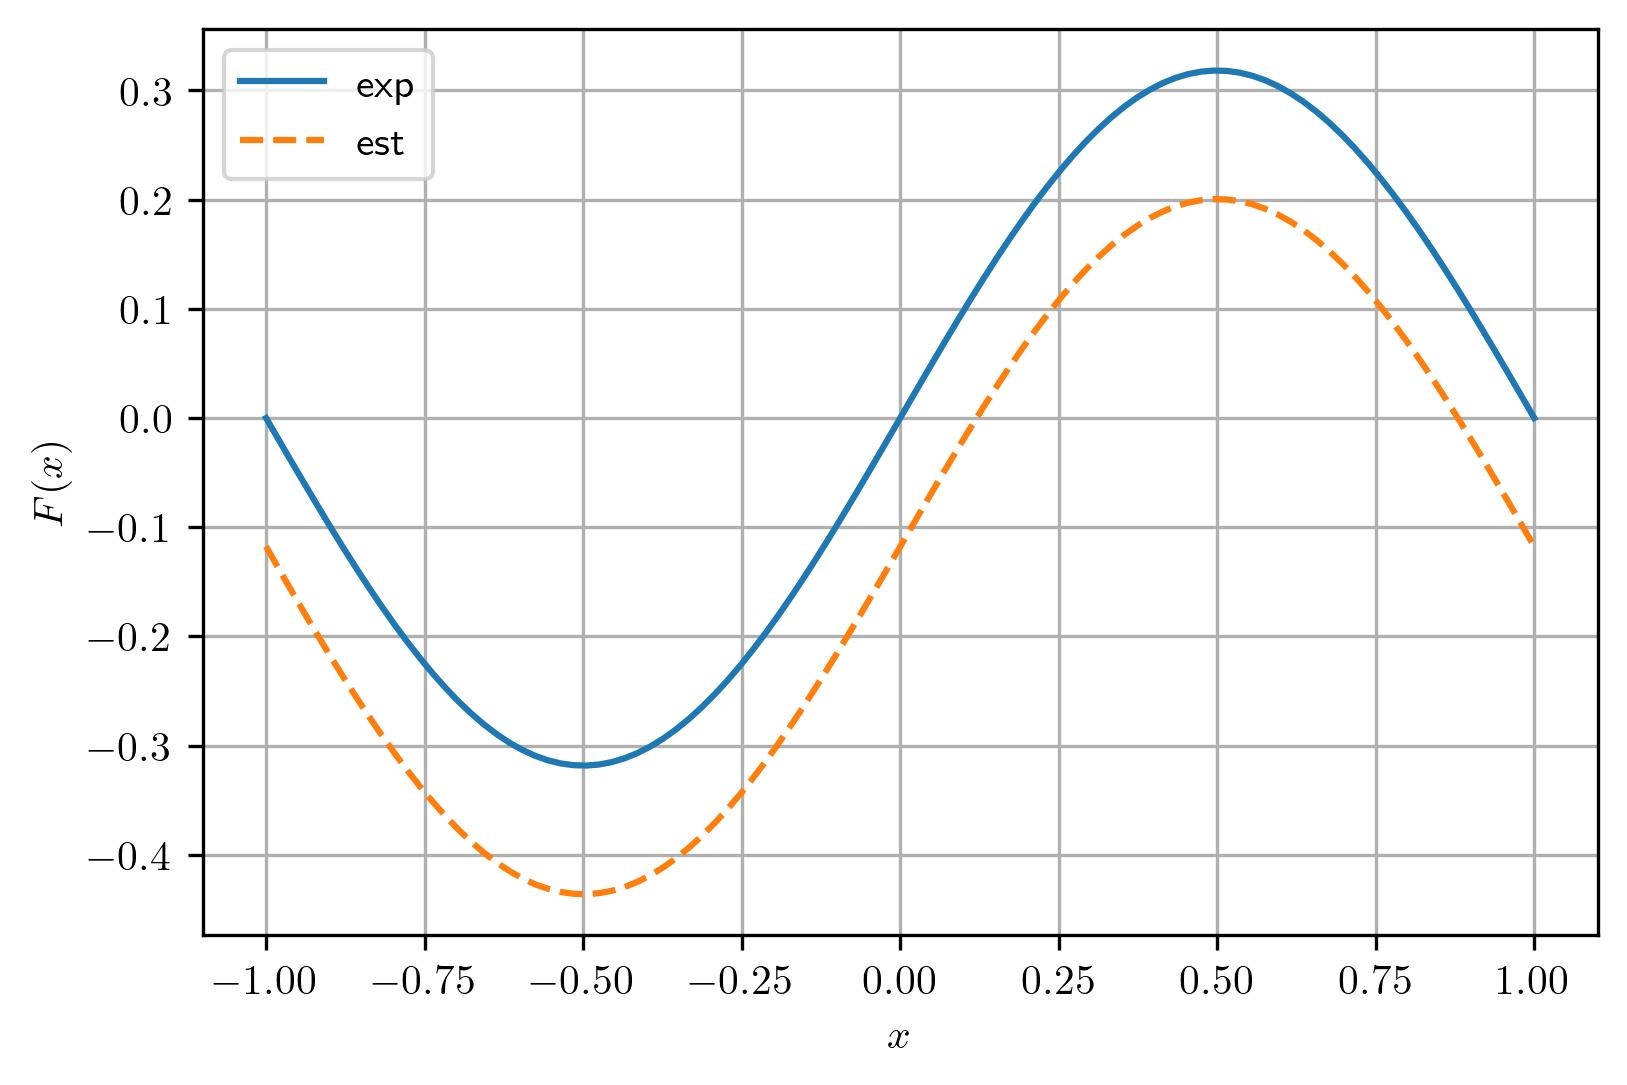
\includegraphics[width=4.5in]{./cap_pinns/dados/ex_integr/fig.jpg}
  \caption{Computação da primitiva de $\cos(\pi x)$ no intervalo de $[-1, 1]$. Linha contínua: valores esperados $y = \frac{1}{\pi}\sen(\pi x)$, para $C = 0$. Linha tracejada: valores estimados $y = \mathcal{N}(x)$.}
  \label{cap_pinns_sec_integr:fig:ex_integr}
\end{figure}

  Neste caso, podemos verificar a solução, uma vez que
  \begin{equation}
    \int_{-1}^{x} \cos(\pi u)\,du = \frac{1}{\pi}\sen(\pi x) + C,
  \end{equation}
  onde $C$ é uma constante arbitrária. Na Figura~\ref{cap_pinns_sec_integr:fig:ex_integr}, temos uma comparação entre o resultado estimado pela rede e o esperado. Observamos que a cada treinamento, a rede pode fornecer uma primitiva diferente.
\end{ex}


%resposta dos exercícios
\ifisbook


\chapter*{Resposta dos Exercícios}\label{cap_respostas}
\addcontentsline{toc}{chapter}{Respostas dos Exercícios}

\shipoutAnswer
\fi

% endnotes
\clearpage
\phantomsection
\addcontentsline{toc}{chapter}{Notas}
\theendnotes

%%references
\ifisbook
\clearpage
\phantomsection
\renewcommand\bibname{Referências}
\addcontentsline{toc}{chapter}{\bibname}
\fi

\begin{thebibliography}{99}

  \bibitem{Agirseven2010a}
    A\u{g}irseven, D., Özi\c{s}, T.. \textit{An analytical study for Fisher type equations by using homotopy   perturbation method}, Computers and Mathematics with Applications, vol. 60, p. 602-609, 2010. \texttt{DOI: \href{http://dx.doi.org/10.1016/j.camwa.2010.05.006}{10.1016/j.camwa.2010.05.006}}

  \bibitem{Goodfellow2016a}
    Goodfellow, I., Bengio, Y., Courville, A.. Deep learning, {MIT} Press, Cambridge, {MA}, 2016.

  \bibitem{Haykin2005a}
    Neural Networks: A Comprehensive Foundation, Haykin, S.. Pearson:Delhi, 2005. ISBN: \texttt{978-0020327615}.

  \bibitem{Raissi}
    Raissi, M., Perdikaris, P., Karniadakis, G.E.. Physics-informed neural networks: A deep learning framework for solving forward and inverse problems involving nonlinear partial differential equations. Journal of Computational Physics 378 (2019), pp. 686-707. DOI: \texttt{10.1016/j.jcp.2018.10.045}.

  \bibitem{Mata}
    Mata, F.F., Gijón, A., Molina-Solana, M., Gómez-Romero, J.. Physics-informed neural networks for data-driven simulation: Advantages, limitations, and opportunities. Physica A: Statistical Mechanics and its Applications 610 (2023), pp. 128415. DOI: \texttt{10.1016/j.physa.2022.128415}.

\end{thebibliography}

\end{document}
